% easychair.tex,v 3.4 2015/12/10

\documentclass{easychair}
%\documentclass[EPiC]{easychair}
%\documentclass[debug]{easychair}
%\documentclass[verbose]{easychair}
%\documentclass[notimes]{easychair}
%\documentclass[withtimes]{easychair}
%\documentclass[a4paper]{easychair}
%\documentclass[letterpaper]{easychair}

\usepackage{doc}
\usepackage{comment}
\usepackage{todonotes}
% use this if you have a long article and want to create an index
% \usepackage{makeidx}

% In order to save space or manage large tables or figures in a
% landcape-like text, you can use the rotating and pdflscape
% packages. Uncomment the desired from the below.
%
% \usepackage{rotating}
% \usepackage{pdflscape}

% Some of our commands for this guide.
%
\newcommand{\easychair}{\textsf{easychair}}
\newcommand{\miktex}{MiK{\TeX}}
\newcommand{\texniccenter}{{\TeX}nicCenter}
\newcommand{\makefile}{\texttt{Makefile}}
\newcommand{\latexeditor}{LEd}
\usepackage[ruled]{algorithm}
\usepackage{algpseudocode}
\theoremstyle{theorem}
\newtheorem{theorem}{Theorem}

\usepackage{amsmath}
\usepackage{graphicx}
\usepackage{todonotes}
\usepackage{tabularx}
\usepackage{latexsym}    
\usepackage[ruled]{algorithm}
\usepackage{algpseudocode}
\usepackage{acronym}


\theoremstyle{remark}
\newtheorem*{remark}{Remark}
%\makeindex

%% Front Matter
%%
% Regular title as in the article class.
%
\title{A Driver's License for Autonomous Vehicles:\\ Composable Hybrid Agents and Benchmark Scenarios}


% Authors are joined by \and. Their affiliations are given by \inst, which indexes
% into the list defined using \institute
%
\author{
Matthew O'Kelly\inst{1}
\and
    Houssam Abbas\inst{1}
\and
Soonho Kong \inst{2}
\and
  Aditya Pinapala \inst{1}
\and
 Rahul Mangharam \inst{1}
}

% Institutes for affiliations are also joined by \and,
\institute{
  University of Pennsylvania,
  Philadelphia, PA, U.S.A.\\
  \email{mokelly@seas.upenn.edu, }
  \email{habbas@seas.upenn.edu, }
  \email{pinapala@seas.upenn.edu}
  \email{rahulm@seas.upenn.edu}
  \and 
  Carnegie Mellon University
  Pittsburgh, PA, U.S.A.
  \email{soonhok@cs.cmu.edu}
}

  
 

%  \authorrunning{} has to be set for the shorter version of the authors' names;
% otherwise a warning will be rendered in the running heads. When processed by
% EasyChair, this command is mandatory: a document without \authorrunning
% will be rejected by EasyChair

\authorrunning{O'Kelly, Abbas, Kong, Pinapala, and Mangharam}

% \titlerunning{} has to be set to either the main title or its shorter
% version for the running heads. When processed by
% EasyChair, this command is mandatory: a document without \titlerunning
% will be rejected by EasyChair
\titlerunning{A Driver's License for Autonomous Vehicles...}

\begin{document}

\maketitle

\begin{abstract}
  To do...
\end{abstract}

% The table of contents below is added for your convenience. Please do not use
% the table of contents if you are preparing your paper for publication in the
% EPiC series

%\setcounter{tocdepth}{2}
%{\small
%\tableofcontents}

%\section{To mention}
%
%Processing in EasyChair - number of pages.
%
%Examples of how EasyChair processes papers. Caveats (replacement of EC
%class, errors).

%\pagestyle{empty}
%------------------------------------------------------------------------------
\section{Outline}
\begin{itemize}
\item Autonomous vehicles are awesome blurb

\item Big challenge in verifying the vehicle's operation between the levels of behavioral planning and trajectory tracking, inclusive. 
\item Source of challenge: variations in physical environment (road networks and regulations), variations in other vehicles (number and behavior), errors of ego vehicle state estimation.
\item We present three benchmarks, which we call scenarios, and preliminary experience in running dReach to verify them.
\item Why reachability rather than, say, stochastic simulation?
\item Ego vehicle model: given a reference trajectory, bicycle model ODE. Environment mode contains reference trajectories for the center of the lane. 
\item Reference trajectory is generated by pure pursuit. 
\item Target point for pure pursuit is generated by hybrid automaton behavioral planner.
\item Other vehicle models
\item Scenario 1: 2 cars on straight road, lane changing.
Describe road network, agents, properties to be satisfied, one dReach run on it.
dReach run results include time bound on verification, tool runtime, number of jumps, number of time steps/jump (?)
\item Scenario 2: 3 cars on curved road. 
Describe same as above.
Then describe 3 successively more complex configurations of that same scenario, but in less detail.
\item Scenario 3: General description of traffic light. Highlight the need for composable agent models. Can no longer hand design verification instance. 
\item Extensions of benchmarks: what can be added to the models to make them more realistic?
\end{itemize}

%------------------------------------------------------------------------------
\section{Introduction}
\label{sect:introduction}

\begin{itemize}
	\item NHTSB says AV software is considered a driver. How does one bound the risk posed to society by software agent. 
	\item Driver's license is a set of tests, we attempt to generalize human behavior based on tests
	\item AV's don't necessarily fail in predictable ways, tests cover an infitesimal portion of the state space, need to gain confidence that algorithms are sound.
	\item Verification Methods and Tools
	\begin{itemize}
		\item Industry Perspective: Testing and Simulation
		\item Control Perspective: Lyapunov Functions
		\item Software Perspective: Model Checking
		\item Logic Perspective: Theorem Proving
	\end{itemize}
\end{itemize}
CPS perspective is an integrated approach that captures the manifestation of errors in the physical world. At its heart is the use of formal models of system and precise mathematical specifications of desired behavior. We are interested in developing the appropriate formal models, a set of specifications, and a battery of scenarios. The community needs to investigate how such methods scale, or fail to scale, and provide new solutions.

\begin{figure}
	\centering
	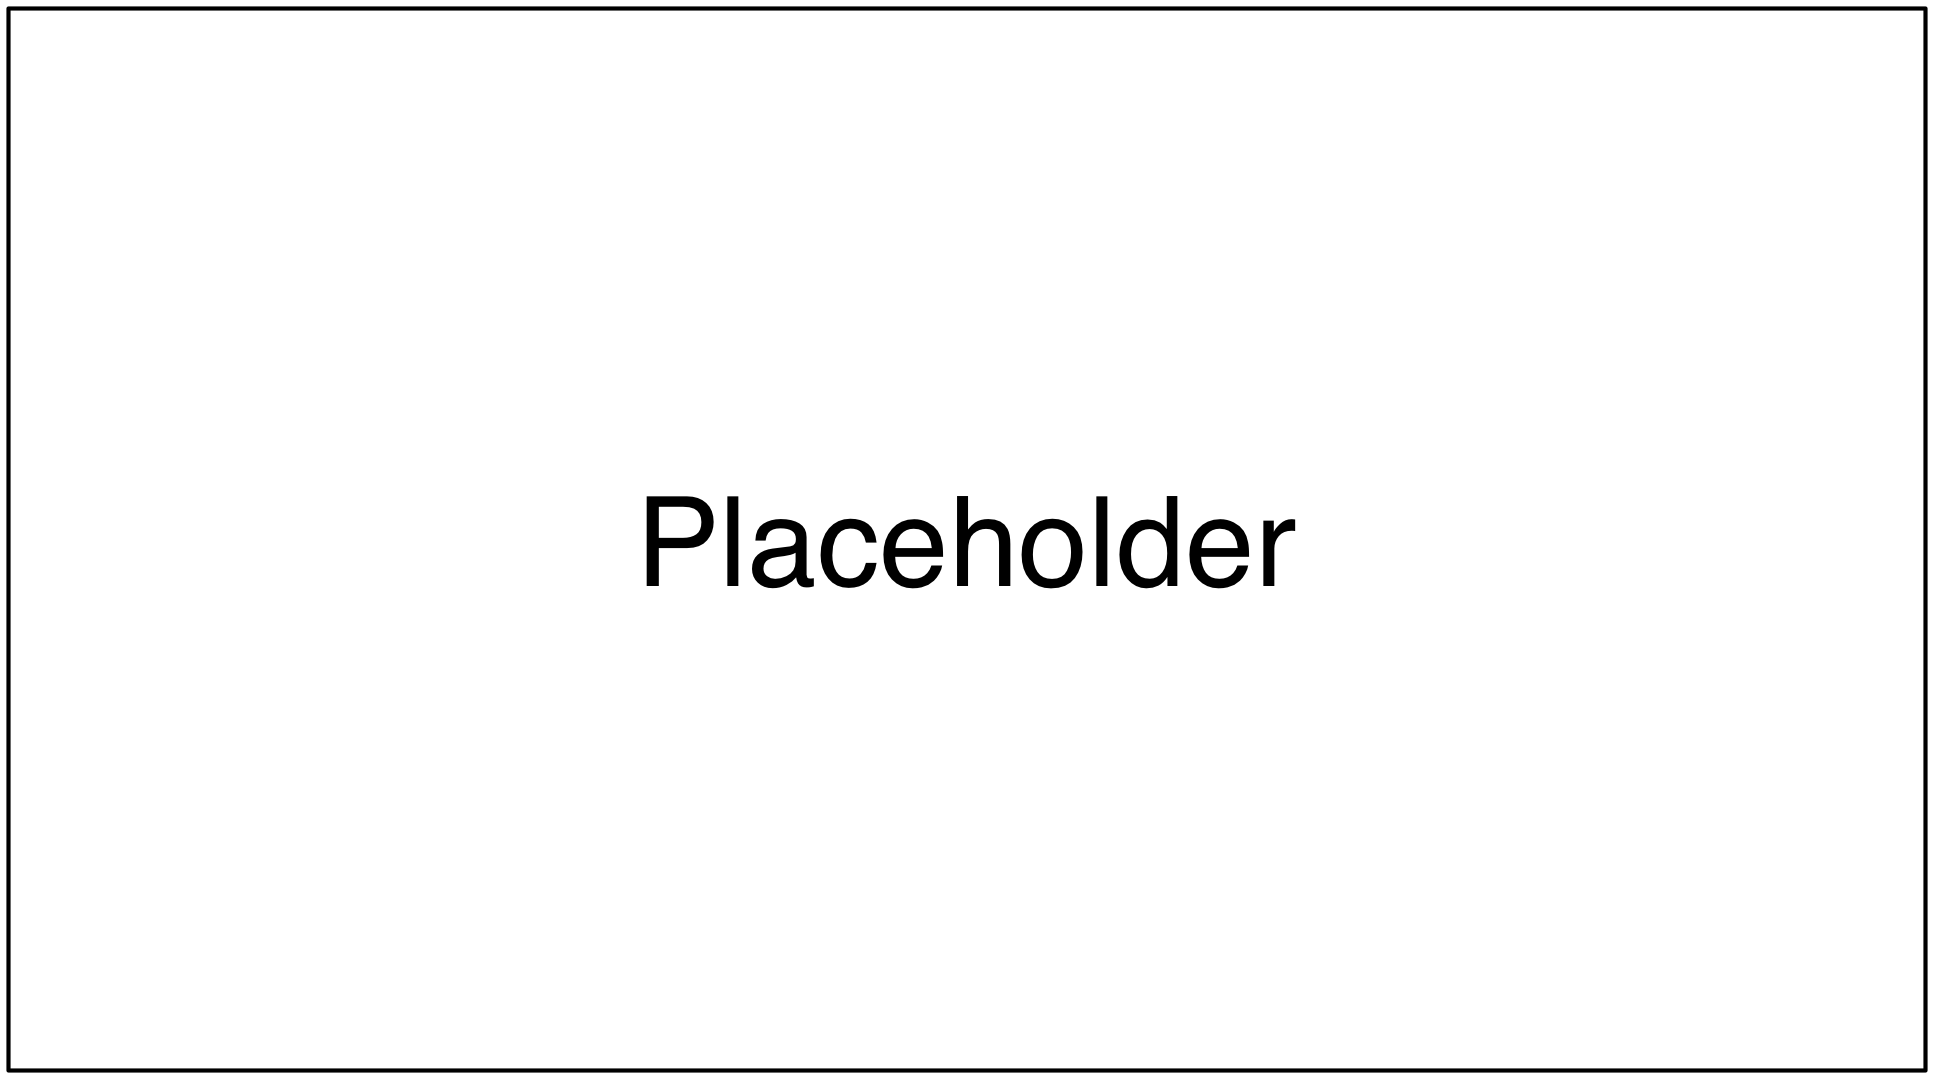
\includegraphics[scale=0.5]{figures/placeholder}
	\caption{A grid of canonical driving scenarios which a human driver might encounter in a certification procedure, highlighted, scenarios covered in this benchmark set}
\end{figure}

%------------------------------------------------------------------------------
\section{Models}
\label{sect:model}
%\emph{Key new idea:} Examine continuous evolution of ego-vehicle, but only discrete evolution of environment. Give environment grid-based abstraction. We don't know the control inputs for the environment anyway\newline
%\emph{Re-examine grid based timed automaton:} Can't really capture accelerations and nuance? 
%\begin{itemize}
%	\item Perception
%	\item Computation and Scheduling
%	\item Traffic Participants
%\end{itemize}
\begin{figure}
	\centering
	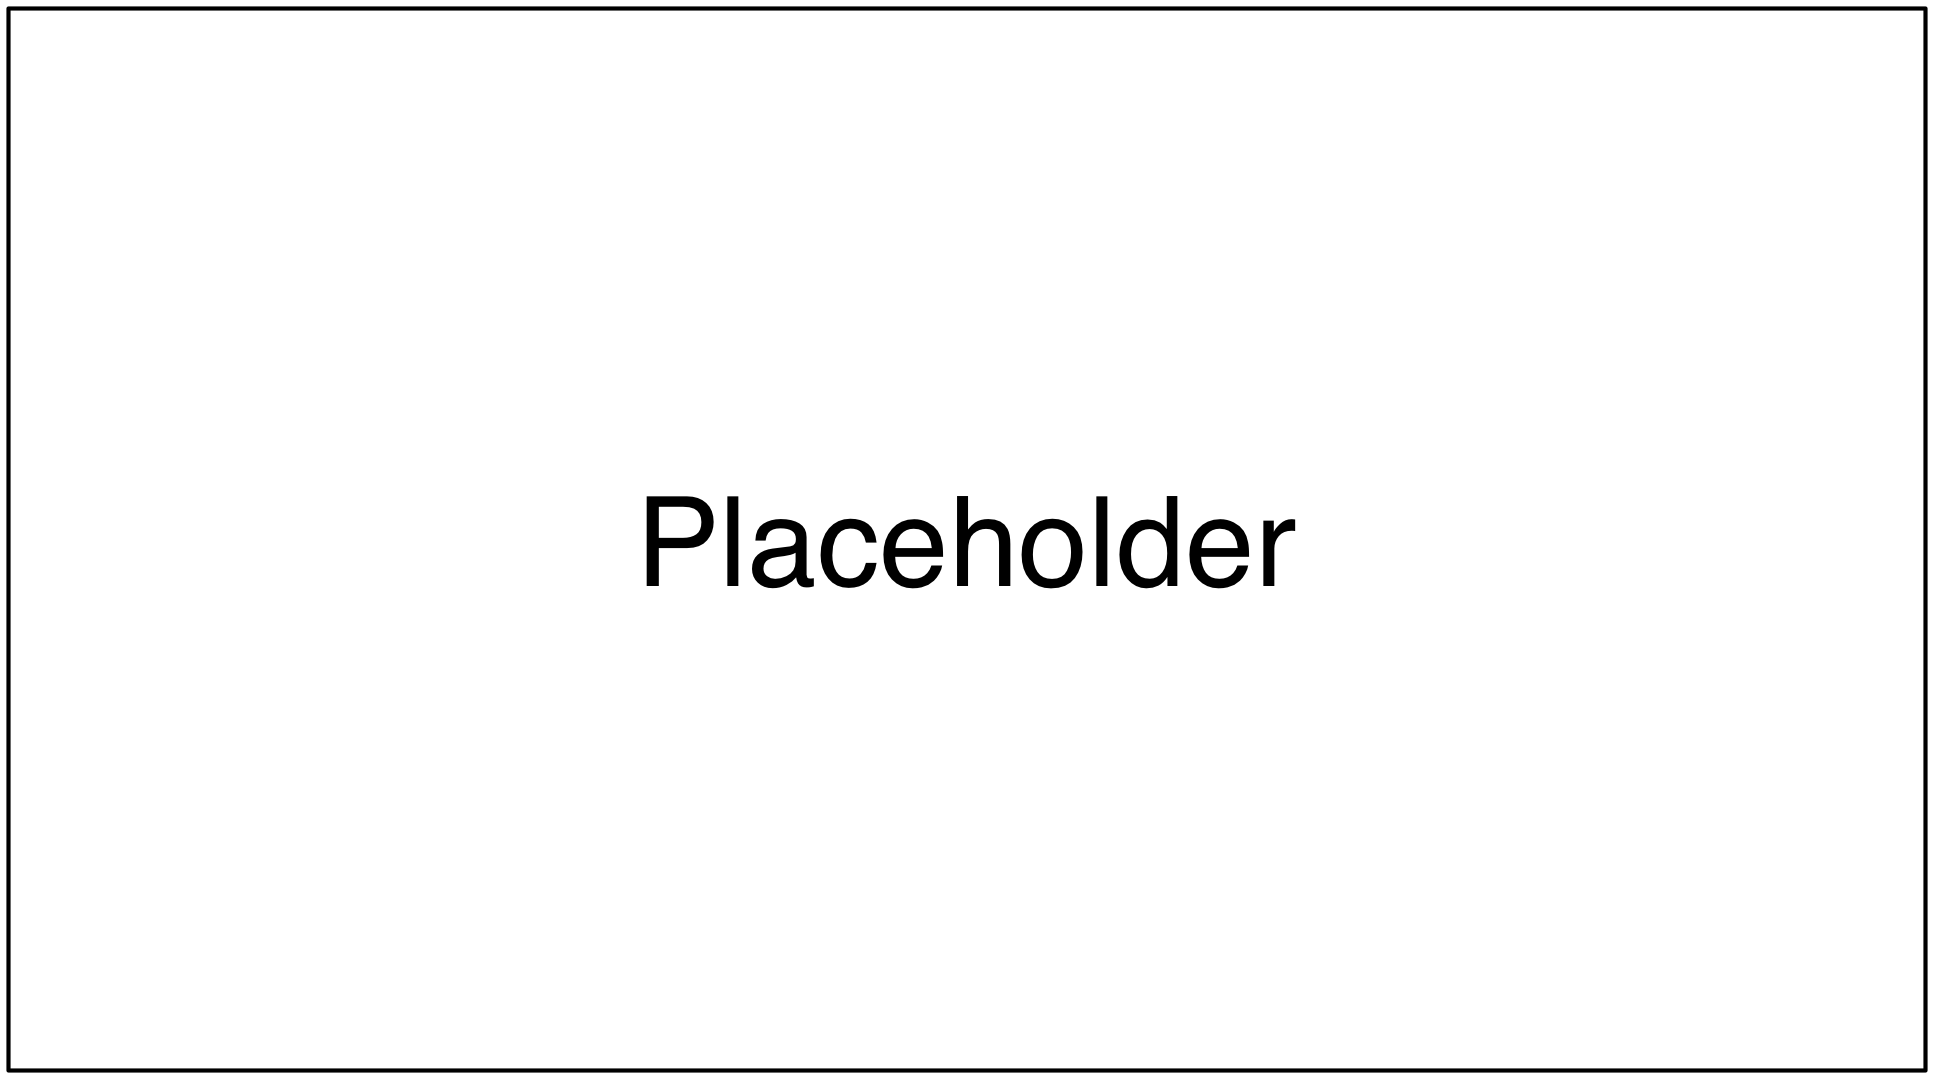
\includegraphics[scale=0.5]{figures/placeholder}
	\caption{Abstraction of Autonomous Driving, APEX preserves... APEX hides...}
\end{figure}
\subsection{Vehicle}
APEX uses a non-linear 7 degree of freedom bicycle model \cite{Rajamani2011} in order to describe the ego-vehicle. 
Higher order models can be supported in the future, and of course the parameters of the base model can be customized in order to match specific vehicles. 
See Fig. \ref{fig:bike}. 
The input to such a model is steering angle velocity and linear velocity, the output is vehicle state as a function of time. 

\begin{figure}[b]
	\centering
	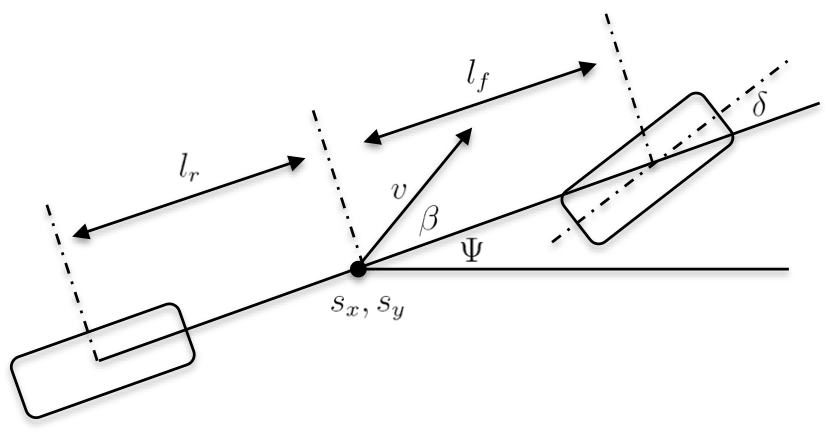
\includegraphics[scale=.5]{figures/bicycle_model}
	\caption{Nonlinear bicycle model describing the statespace for the APEX approach to vehicle dynamics}
	\label{fig:bike}
\end{figure}

The state vector describing the vehicle is described in equations (1)-(7). 
The variable \(\beta\) is the slip angle at the center of mass, \(\psi\) is the heading angle, \(\dot{\psi}\) is the yaw rate, \(v\) is the velocity, \(s_x\) and \(s_y\) are the x and y positions, and \(\delta\) is the angle of the front wheel. In the formulation of [6], the inputs to the system are \(a_x\), the longitudinal acceleration, and \(v_w\) the rotational speed of the steering angle. 
%The \(y\) terms represent disturbances to the system. For example \(y_{\beta}\) and \(y_{\dot{\psi}}\) represent disturbances to the slip angle at the center of mass and the yaw rate. 
\begin{equation}
x_v = (\beta,\Psi,\dot{\Psi}, v, s_x, s_y, \delta)
\end{equation}	
The state equations for the system as described in \cite{Althoff2014} are:
\begin{equation}
\label{eqn:beta}
\dot{\beta}=\left(\frac{C_rl_r-C_fl_f}{mv^2} \right)\dot{\psi}+\left(\frac{C_f}{mv} \right)\delta-\left(\frac{C_f+C_r}{mv} \right)\beta
\end{equation}
\begin{gather}
\label{eqn:psi}
\ddot{\psi}=\left(\frac{C_rl_r-C_fl_f}{I_z} \right)\beta-\left(\frac{C_fl_f^2-C_rl_r^2}{I_z} \right)\left(\frac{\dot{\psi}}{v} \right) \notag \\
+\left(\frac{C_fl_f}{I_z} \right)\delta
\end{gather}
\begin{equation}
\label{eqn:v}
\dot{v}=a_x
\end{equation}
\begin{equation}
\label{eqn:sx}
\dot{s_x}=v\cos{(\beta+\psi)}
\end{equation}
\begin{equation}
\label{eqn:sy}
\dot{s_y}=v\sin{(\beta+\psi)}	
\end{equation}	
\begin{equation}
\label{eqn:delta}
\dot{\delta}=v_w
\end{equation}

%We note that in order to analyze the system we represent \(\ddot{\psi}\) as two first order differential equations. Thus we write:
%\begin{gather}
%	\dot{\psi}_{dot}=\left(\frac{C_rl_r-C_fl_f}{I_z} \right)\beta-\left(\frac{C_fl_f^2-C_rl_r^2}{I_z} \right)\left(\frac{\dot{\psi}}{v} \right) \notag \\+\left(\frac{C_fl_f}{I_z} \right)\delta\\
%	\dot{\psi}=\psi_{dot}
%\end{gather}
%Finally, one must substitute \(\psi_{dot}\) for each appearance of \(\dot{\psi}\) in the other state equations.

\subsubsection{Vehicle Parameters}
The parameters \(C_f,C_r\) and \(l_f, l_r\) describe respectively the cornering stiffness and distances from the center of gravity to the axles respectively; the subscripts $f,r$ denote whether the parameter is defined for the front or rear of the vehicle. The moment of inertia, \(I_z\) and the vehicle mass, \(m\) are experimentally determined constants \cite{Snider2009}. 
The kinematic bicycle model considers the two front wheels and two rear wheels of the vehicle to move in unison, with steering provided by the front wheels only. Furthermore, Each abstracted wheel is located along the center of the vehicle's body. Table \ref{table:vehiclep} contains the validated vehicle parameters as given in \cite{Althoff2014}. It is possible to obtain such parameters and replace these constants in order to investigate specific vehicle characteristics. 

\begin{table}[h]
	\centering
	\caption{Parameters of Example Ego Vehicle \cite{Althoff2014}}
	\label{table:vehiclep}
	\begin{tabular}{|c|c|c|c|c|c|}
		\hline
		\multicolumn{6}{|c|}{Vehicle Parameters} \\ \hline
		\textit{$m$(kg)} & \textit{$I_z$(kg*m$^2$)} & \textit{$C_f$(N/rad)} & \textit{$C_r$(N/rad)} & \textit{$l_f$(m)} & \textit{$l_r$(m)} \\ \hline
		2273 & 4423 & 10.8e4 & 10.8e4 & 1.292 & 1.515 \\ \hline
	\end{tabular}	
\end{table}


\subsubsection{Pure Pursuit}
The simplest algorithm for path tracking and trajectory generation...
From a type perspective what is the difference between arc and spline? 
Geometrically, the arc satisfies \textbf{convexity}. 
\begin{itemize}
	\item Given a current position at the vehicles rear differential and a goal...
	\item The algorithm computes a constant curvature arc between the current position and the goal.
	\item The vehicle may then actuate its steering system such that the curvature of the arc is tracked.
	\item Downside is discontinuity between curvatures when the algorithm is iterated
	\item Is also reliant on waypoints, does not generate alternate maneuvers unless explicitly told to switch goals. 
\end{itemize}
\textbf{Algorithm:}
\begin{itemize}
	\item Update vehicle state
	\item Find nearest path point
	\item Find the goal point
	\item Transform goal to vehicle coordinates
	\item Calculate desired curvature
	\item Set steering to desired curvature
	\item Update position
\end{itemize}
\begin{figure}
	\centering
	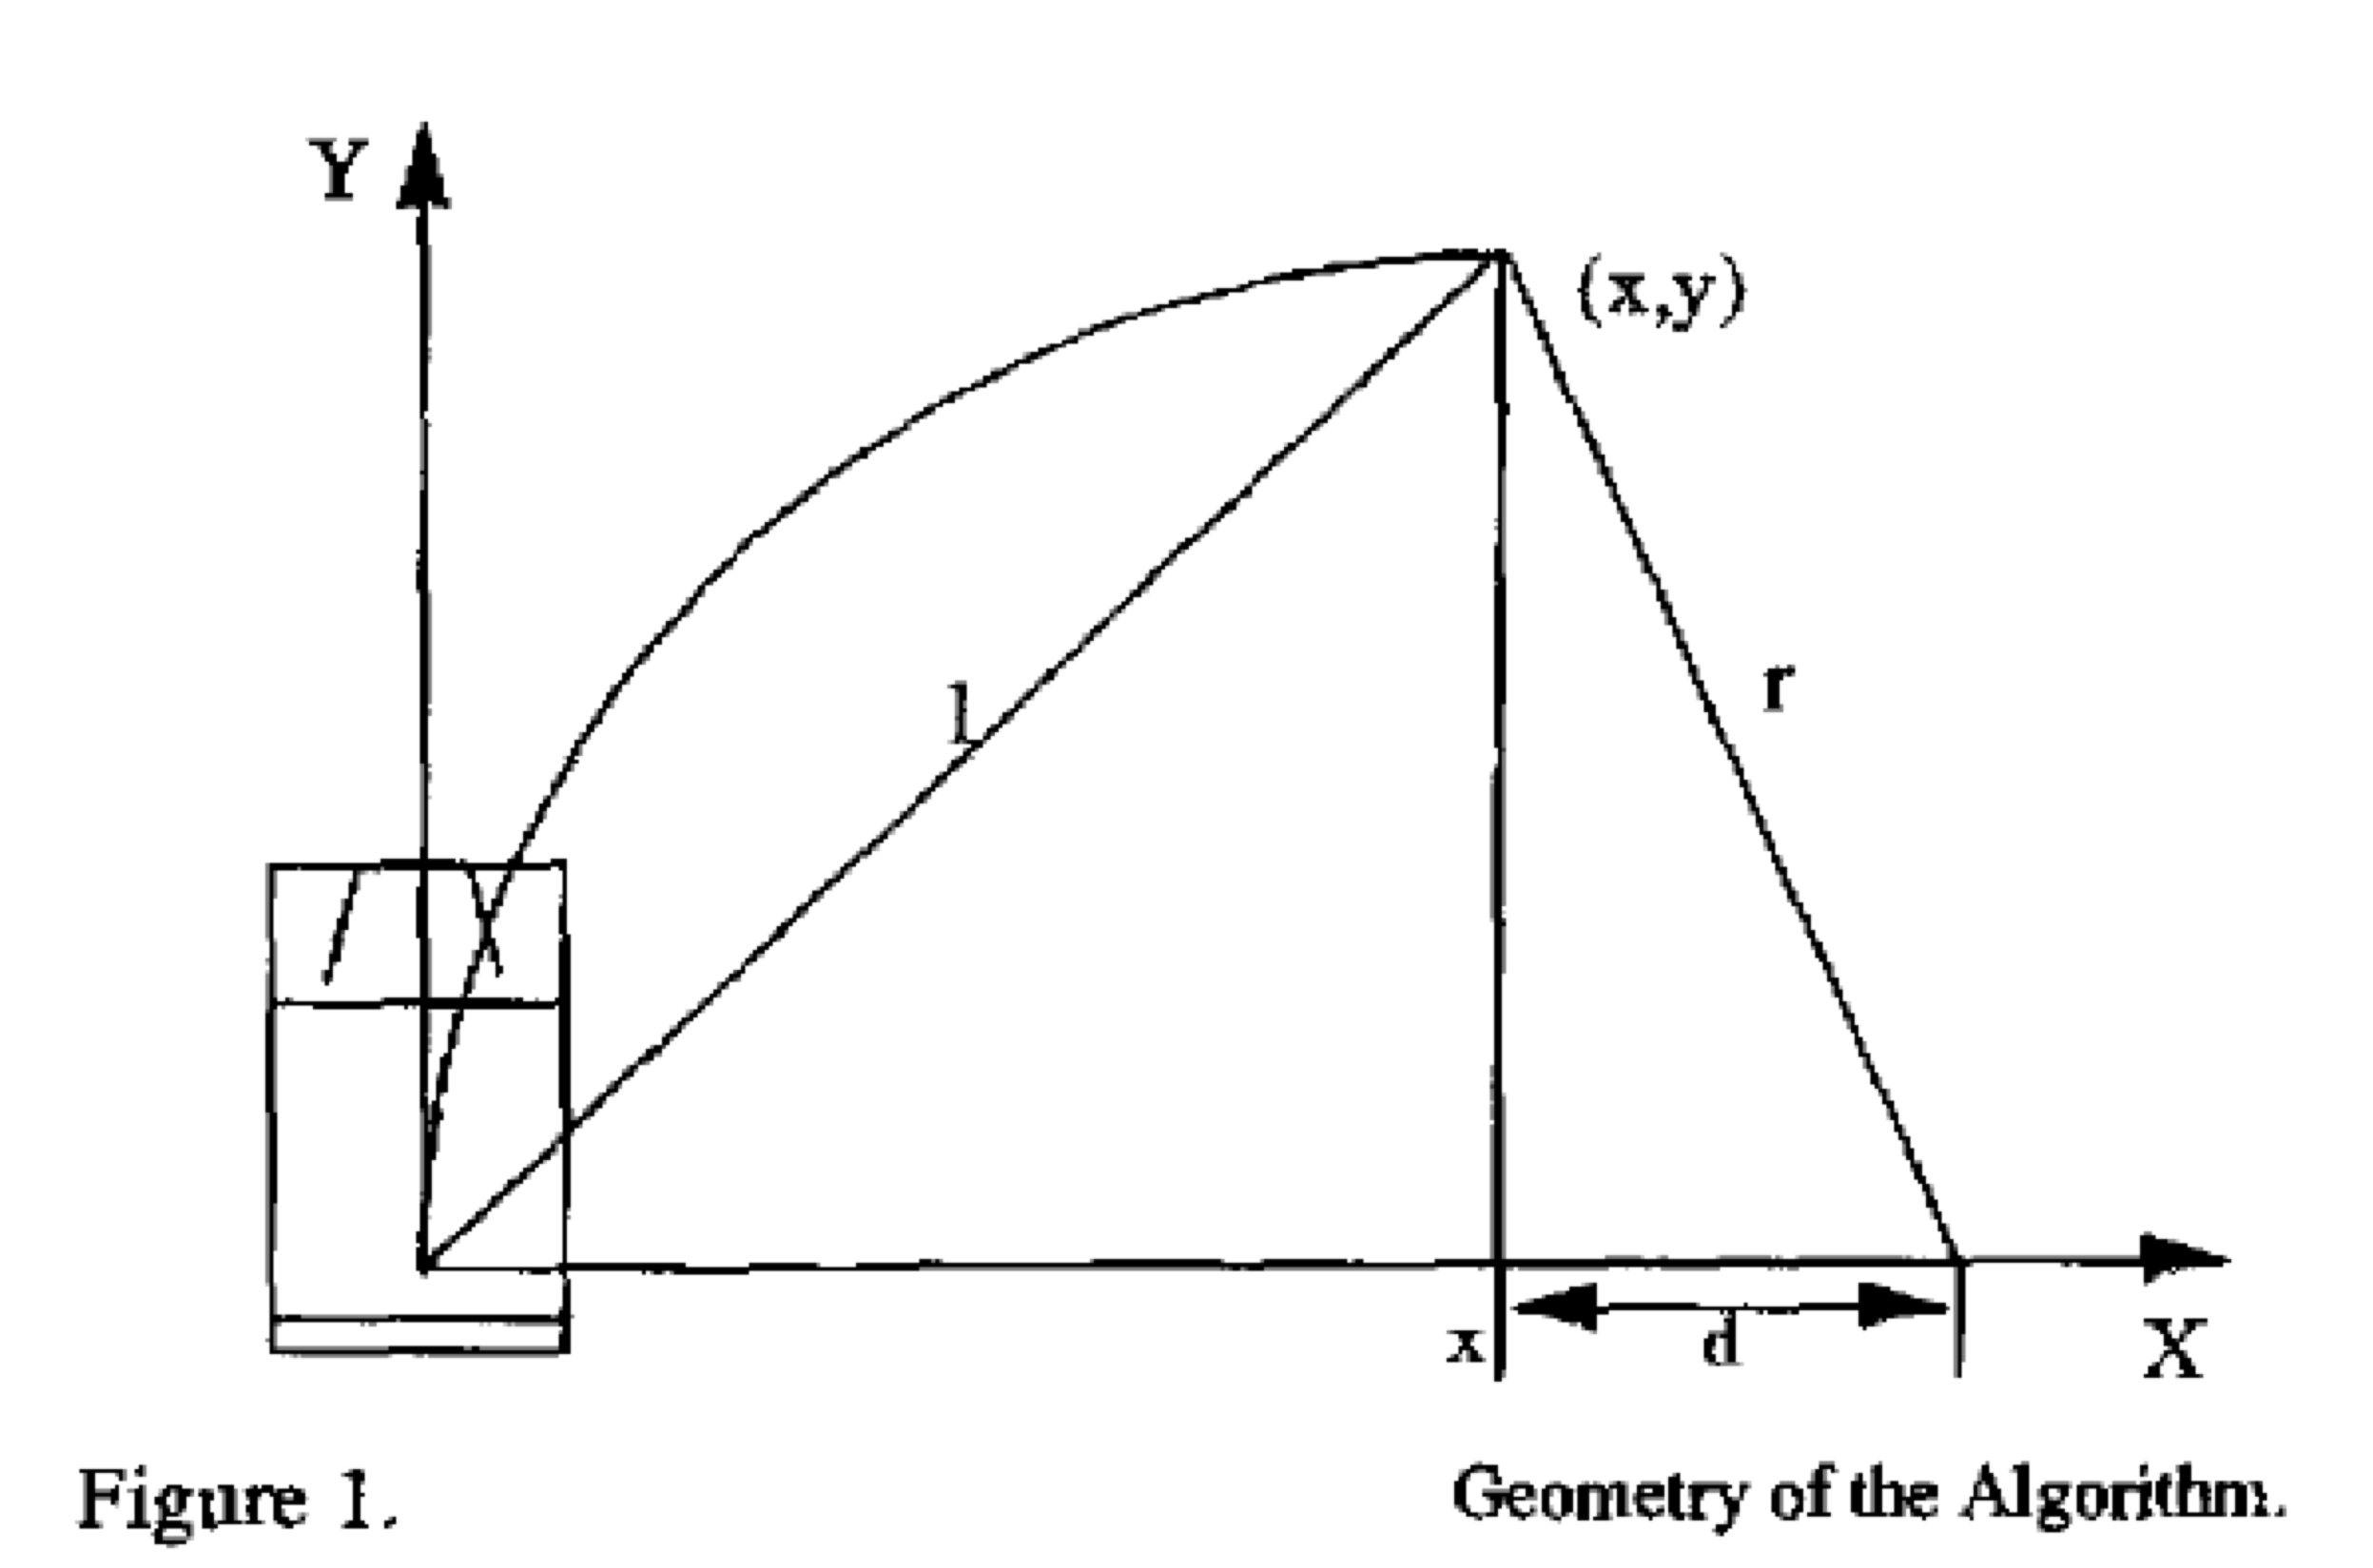
\includegraphics[scale=.5]{figures/pure_pursuit_geom}
	\caption{Geometry of Pure Pursuit Algorithm}
\end{figure}
\begin{align}
x^2+y^2=l^2\\
x+d=r
\end{align}

\noindent Now for the curvature such that:
\begin{align}
r=\frac{l^2}{2x}\\
\gamma=\frac{2x}{l^2}
\end{align}

\subsubsection{Tracking Controller}
A simple trajectory tracking controller is included with the APEX vehicle model. Trajecotry tracking controllers guide a vehicle along a geometrically defined cubic spline by apply steering and longitudinal acceleration inputs. A successful path tracking algorithm maintains vehicle stability and attempts to minimize the error between the desired trajectory and actual trajectory. The parameters computed for this controller when implemented and validated on a typical crossover SUV \cite{Althoff2014} are presented in Table \ref{table:controller}. 

\begin{table}[h]
	\centering
	\caption{Controller Parameters \cite{Althoff2014}}
	\label{table:controller}
	\begin{tabular}{|c|c|c|c|c|c|}
		\hline
		\multicolumn{6}{|c|}{Controller Parameters} \\ \hline
		$k_1$ & $k_2$ & $k_3$ & $k_4$ & $k_5$ & $k_6$ \\ \hline
		2 & 12 & 4 & 2 & 1 & 1.515 \\ \hline
	\end{tabular}	
\end{table}

Using the approach in \cite{Snider2009} and \cite{Althoff2014} the control inputs for longitudinal acceleration (pressing the accelerator) and steering angle velocity (turning the steering wheel) can be computed as $v_w$ and $a_x$ respectively. 

\begin{gather}
v_w=k_1(cos{(\Psi_d)}(s_{y,d}-s_y-w_y)-sin{(\Psi_d)}(s_{x,d}-s_x-w_x)) \notag \\ +k_2(\Psi_d-\Psi-w_{\Psi}) \notag \\ +k_3(\dot{\Psi_d}-\dot{\Psi}-w_{\psi})-k_4(\delta-w_{\delta})
\\
a_x=k_5(cos{(\Psi_d)}(s_{x,d}-s_x-w_x)+sin{(\Psi_d)}(s_{y,d}-s_y-w_y)) \notag \\ +k_6(v_d-v-w_v)
\end{gather}

%Thus, the feedback to the system are the lateral and longitudinal tracking errors. We derive the following results as in  \cite{Snider2009}:
%\begin{gather}
%	\epsilon_x=cos{(\Psi_d)}(s_{x,d}-s_x) +sin{(\Psi_d)}(s_{y,d}-s_y)
%	\\
%	\epsilon_y=-sin{(\Psi_d)}(s_{x,q}-s_x)+cos{(\Psi_d)}(s_{y,d}-s_y)
%\end{gather}

Given that the ego-vehicle will be following constant curvature arcs defined by the pure-pursuit method. We must compute $\left\{\Psi_d, \dot{\Psi}_d, s_{x_d}, s_{y_d},\right\}$. 

\noindent We begin by computing the initial orientation of the vehicle:
\begin{equation}
	\Psi_d (0) = \frac{\pi}{2}- \theta(0)
\end{equation}
We note $\theta(0)$ can be computed via this simple relation:
\begin{equation}
	sin(\theta(0)) = \frac{s_y-c_y}{r}
\end{equation}
This implies that:
\begin{equation}
	\theta(0) = sin^{-1} \left(\frac{s_y-c_y}{r}\right)
\end{equation}
Then we compute 
\begin{equation}
\Psi_d(t) =  \frac{\pi}{2}-\theta(t)
\end{equation}
For an arc subtended by the angle $\theta(t)$, the length of the arc, $\rho$ is:
\begin{equation}
	\rho = \theta(t) \cdotp r
\end{equation}
Alternately one might compute the length of the arc by integrating the velocity as directed along the arc such that $\rho(t) = \int_{0}^{t}v(\alpha) d\alpha$. Now we let $v(\alpha) = v_d$ and hold $v_d$ to be constant. Thus:
\begin{equation}
	\rho(t) = v_d \cdotp t
\end{equation}
Which implies that:
\begin{equation}
	\Psi_d(t) = \frac{\pi}{2} - \left( \theta(0) + \frac{v_d \cdotp t}{r}\right)\right)
\end{equation}
Differentiating we conclude that:
\begin{equation}
	\dot{\Psi}_d = -\frac{v_d}{r}
\end{equation}
\begin{figure}
	\centering
	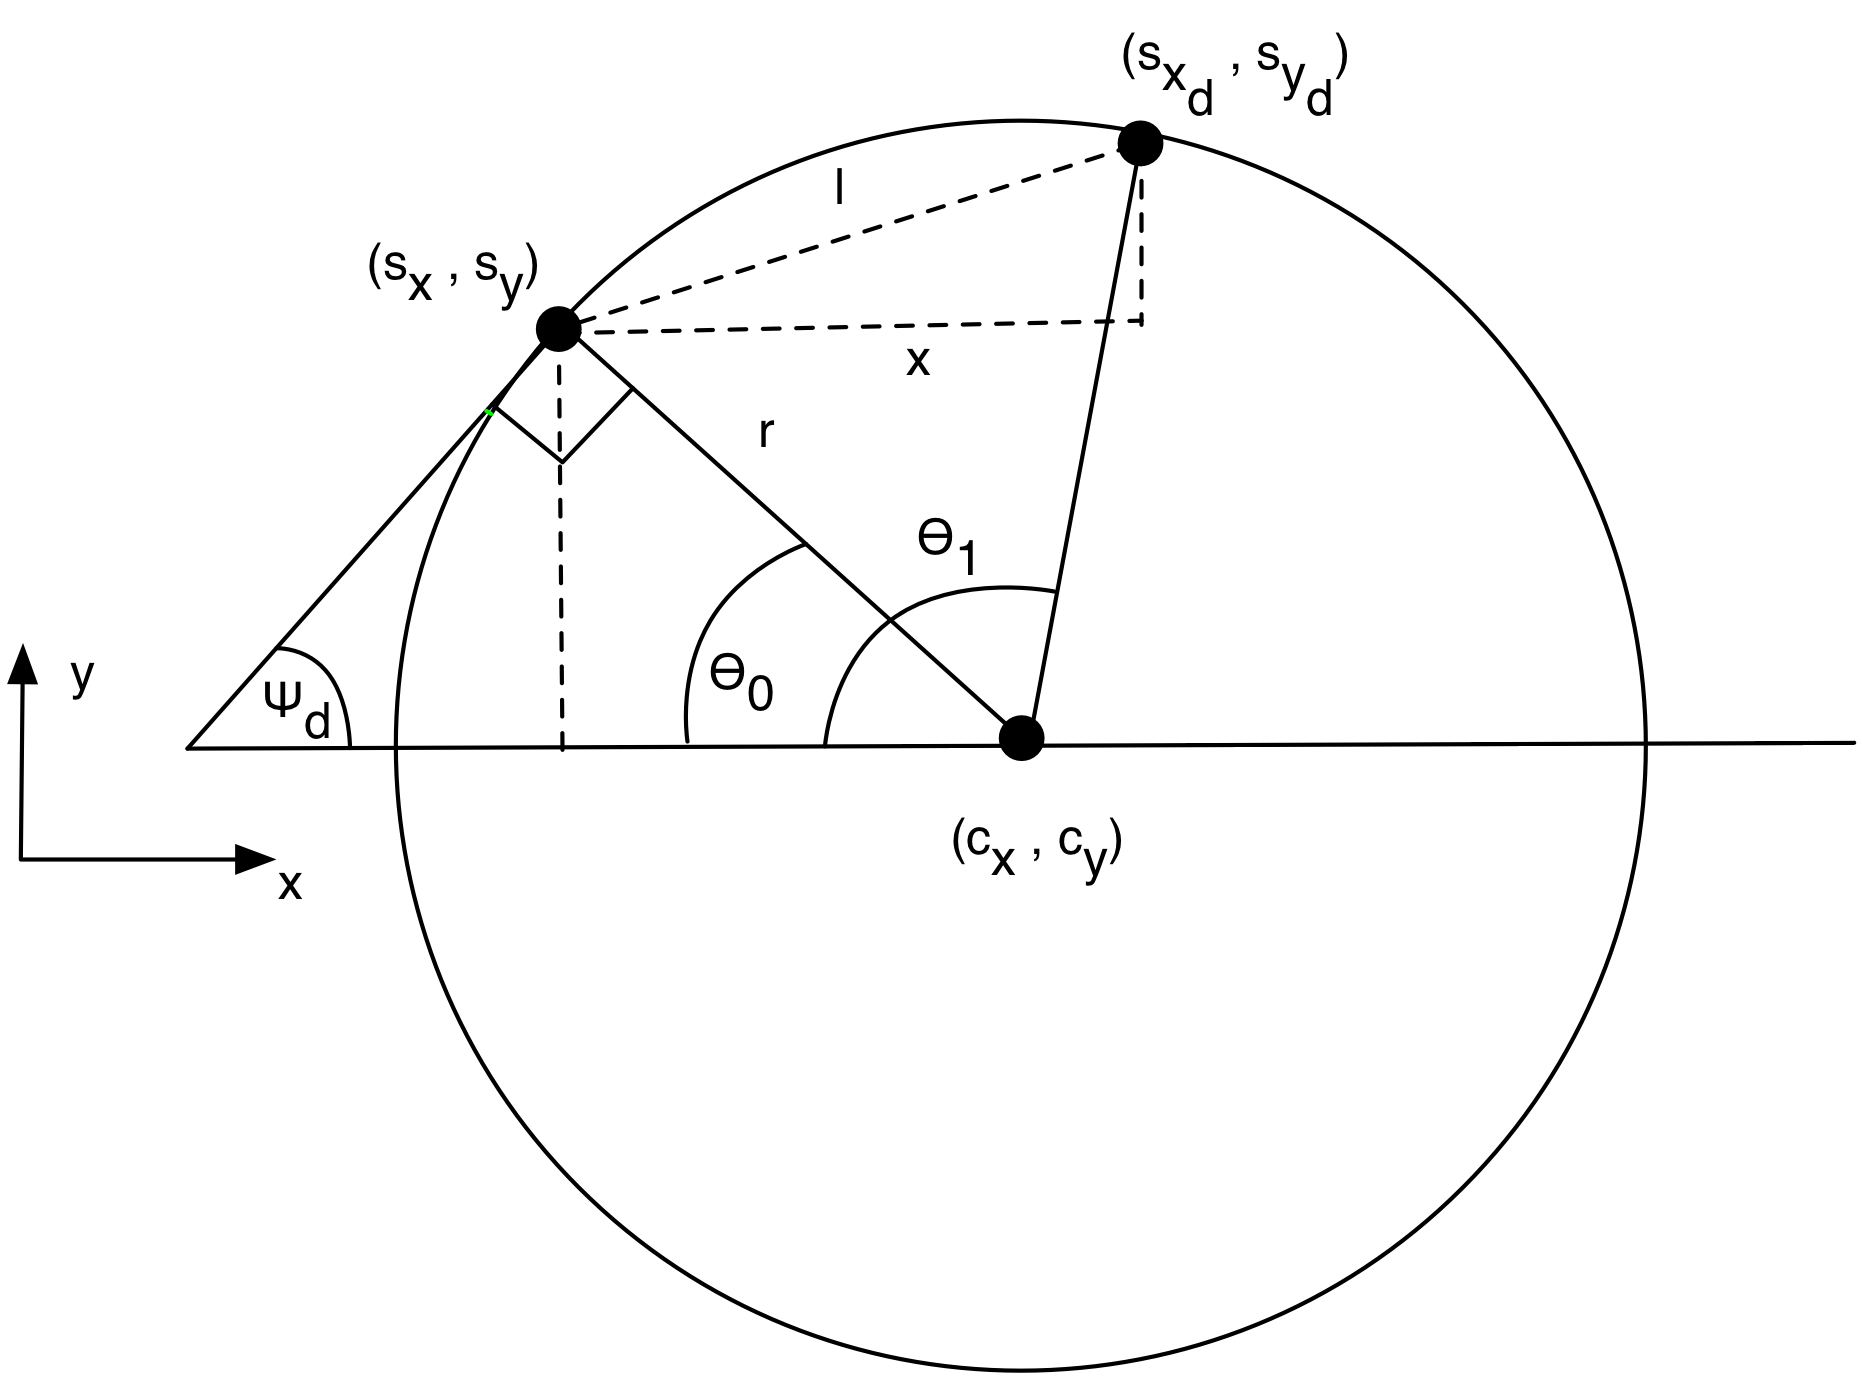
\includegraphics[scale=0.5]{figures/traj-track-diagram}
	\caption{Geometric Description of Ego-Vehicle Trajectory Geometry}
\end{figure}

\noindent Thus we can derive the remaining equations for a point mass moving in a plane:
\begin{gather}
 \dot{\Psi}_d= -v_d/r\\
 \dot{s}_{x_d} = v_d \left(cos(\Psi_d)\right)\\
 \dot{s}_{y_d} = v_d \left(sin(\Psi_d) \right)\\
 \ddot{\Psi}_d = 0
\end{gather}
\subsubsection{Behavioral Controller}

\begin{figure}[h]
	\centering
	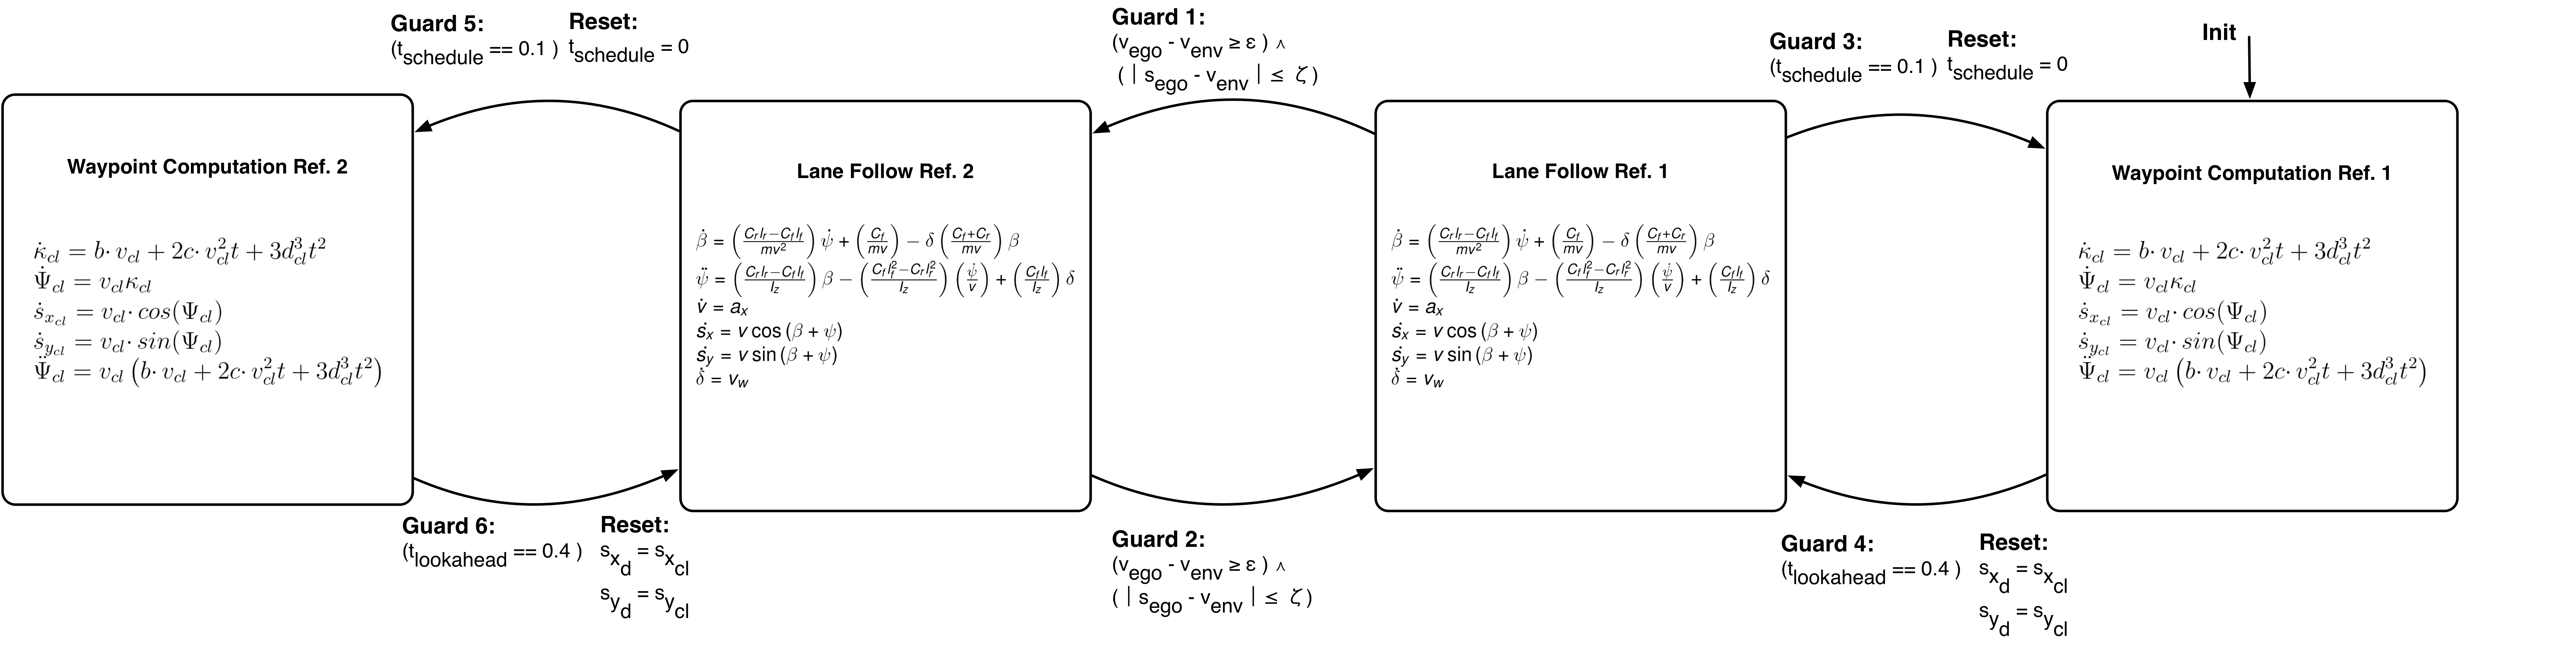
\includegraphics[width=\textwidth]{figures/arch-ego-automaton}
	\caption{The behavioral controller governing the lane selection of the ego-vehicle}
\end{figure}
Define the behavioral controller as an FSM. Can come from anywhere. Example we show is Fig. 6.
\subsection{Road}
High level view of the road is a network of connected segments. Graph describes reachability of one segment from another. Each segment need not be straight etc. We will choose to define segments via a collection of boundary points. 
\subsubsection{Boundaries}
Each segment must have a left and right boundary. The boundaries are defined by an ordered sequence of points. We interpolate linearly between points. 
\subsubsection{Computing Centerline Trajectories}
Each centerline is defined by an ordered sequence of points. In order to come to a continuous representation of the trajectory we interpolate between the points using Cubic splines. This ensures that the centerline trajectory is continuous. We may introduce offset trajectories from the centerline, but do not do so in this work. 
Each execution of the centerline computation we require as an input the current state and a goal state as defined by the ordered sequence of waypoints. This computation is done outside of the verification instance and supplied as part of the environment data. It is clear that this computation can be automated given an annotation of a map supplied by OpenStreetMaps etc.

The ``vehicle" model, a point mass, represents the kinematic constraints which we wish to impose on such an idealized trajectory. We note that we will call the vehicle state $x_{cl}$ because it does not necessarily have to be the same as the model used for verification (although it can be). The centerline represents an ideal trajectory, therefore, lower order models are often substituted here which do not account for control inputs as we are not actually executing a vehicle. In this implementation we define $x_{sl}$ as:
\begin{equation}
x_{sl}=(s_x, s_y, v, \Psi, \kappa)
\end{equation}

Where $s_x$ and $s_y$ are the x and y positions of the center of mass, $v$ is the velocity, $\Psi$ is the heading angle, and $\kappa$ is the curvature. We note that the state equations involve an additional constant, $L$ which is the wheelbase of the vehicle.
Where the state equations are described as:
\begin{equation}
\dot{x}= v*cos(\Psi)
\end{equation}
\begin{equation}
\dot{y} = v*sin(\Psi)
\end{equation}
\begin{equation}
\dot{\theta}= \kappa*v
\end{equation}
\begin{equation}
\dot{\kappa} = \frac{\dot{\Psi}}{L}
\end{equation}

The local planner's objective is then to find a feasible trajectory from the initial state defined by the tuple $x_{sl}$ to a goal pose $x_{p}$ defined as:
\begin{equation}
x_{p} = (s_x,s_y,\Psi)
\end{equation}

In this formulation we limit trajectories to a specific class of parameterized curves known as cubic splines. A cubic spline is defined as a function of arc length:
\begin{equation}
\kappa(s) = \kappa_0 + a \kappa_1 s + b \kappa_2 s^2 + c \kappa_3 s^3
\end{equation}

Note that there are four free parameters $(a,b,c,s_f)$ and our goal posture has four state variables. Thus, a cubic spline is a minimal polynomial that can be assured to produce a trajectory from the current position to the goal position (if it is kinematically feasible). For any particular state, goal pair there are two steps necessary to compute the parameters. First, it is necessary to produce an initial guess. There are several approaches available such as using a neural network, lookup table, or a simple heuristic. In this case we adapt a heuristic from Nagy and Kelly \cite{nagy2001trajectory} such that it is compatible with a stable parameter formulation presented by McNaughton \cite{McNaughton_2011_6927}. The stable reparameterization is defined as:
\begin{gather}
\kappa(0)=p_0\\
\kappa(s_f/3)=p_1\\
\kappa(2s_f/3)=p_2\\
\kappa(s_f)=p_3
\end{gather}

Where the parameters $(a,b,c,s_f)$ can now be expressed as:
\begin{gather}
a(p)=p_0\\
b(p)=-\frac{11p_0 - 18p_1+9p_2-2p_3}{2s_f}\\
c(p)=\frac{9*(2p_0-5p_1+4p_2-p_3)}{2s_f^2}\\
d(p)=-\frac{9(p_0-3p_1 +3p_2-p_3)}{2s_f^3}
\end{gather}
Which results in the following initialization heuristic:
\begin{gather}
p_0=\kappa_0=\kappa_i\\ 
p_1=\kappa_1= \frac{1}{49}(8b(s_f-s_i)-26\kappa_0-\kappa_3)\\
p_2=\kappa_2=\frac{1}{4}(\kappa_3-2\kappa_0+5\kappa_1)\\
p_3=\kappa_3=\kappa_f
\end{gather}
\subsubsection{Computing Goal Points} 
Given a parameterized trajectory, it is only possible to compute the evolution of the vehicle's planning state vector via forward simulation of the point-mass dynamics...
\begin{gather}
	    \dot{\kappa}_{cl} = b\left(v_{cl}\right) + 2c\left(v_{cl}^{2}t\right) + 3d\left(v_{cl}^{3}t^{2}\right) \\
	    \dot{\Psi}_{cl}= v_{cl}\left(\kappa_{cl}\right)	\\
	    \dot{s}_{x_{cl}}= v_{cl}\left(cos(\Psi_{cl})\right)\\
	    \dot{s}_{y_{cl}}= v_{cl}\left(sin(\Psi_{cl})\right)\\
	    \ddot{\Psi}_{cl} =v_{cl} \left( b\left(v_{cl}\right) + 2c\left(v_{cl}^{2}t\right) + 3d\left(v_{cl}^{3}t^{2}\right) \right)	    
\end{gather}
We define a lookahead time $t_{la}$ and forward simulate motion along the centerline trajectory through the dynamics defined above. Having, completed such an operation the next waypoint for the pure pursuit algorithm is simply:

\begin{equation}
	\left(s_{x_{cl}}(t_{la}), s_{y_{cl}}(t_{la})\right)
\end{equation} 

\subsection{Other Vehicles}
	\begin{figure}[h]
		\centering
		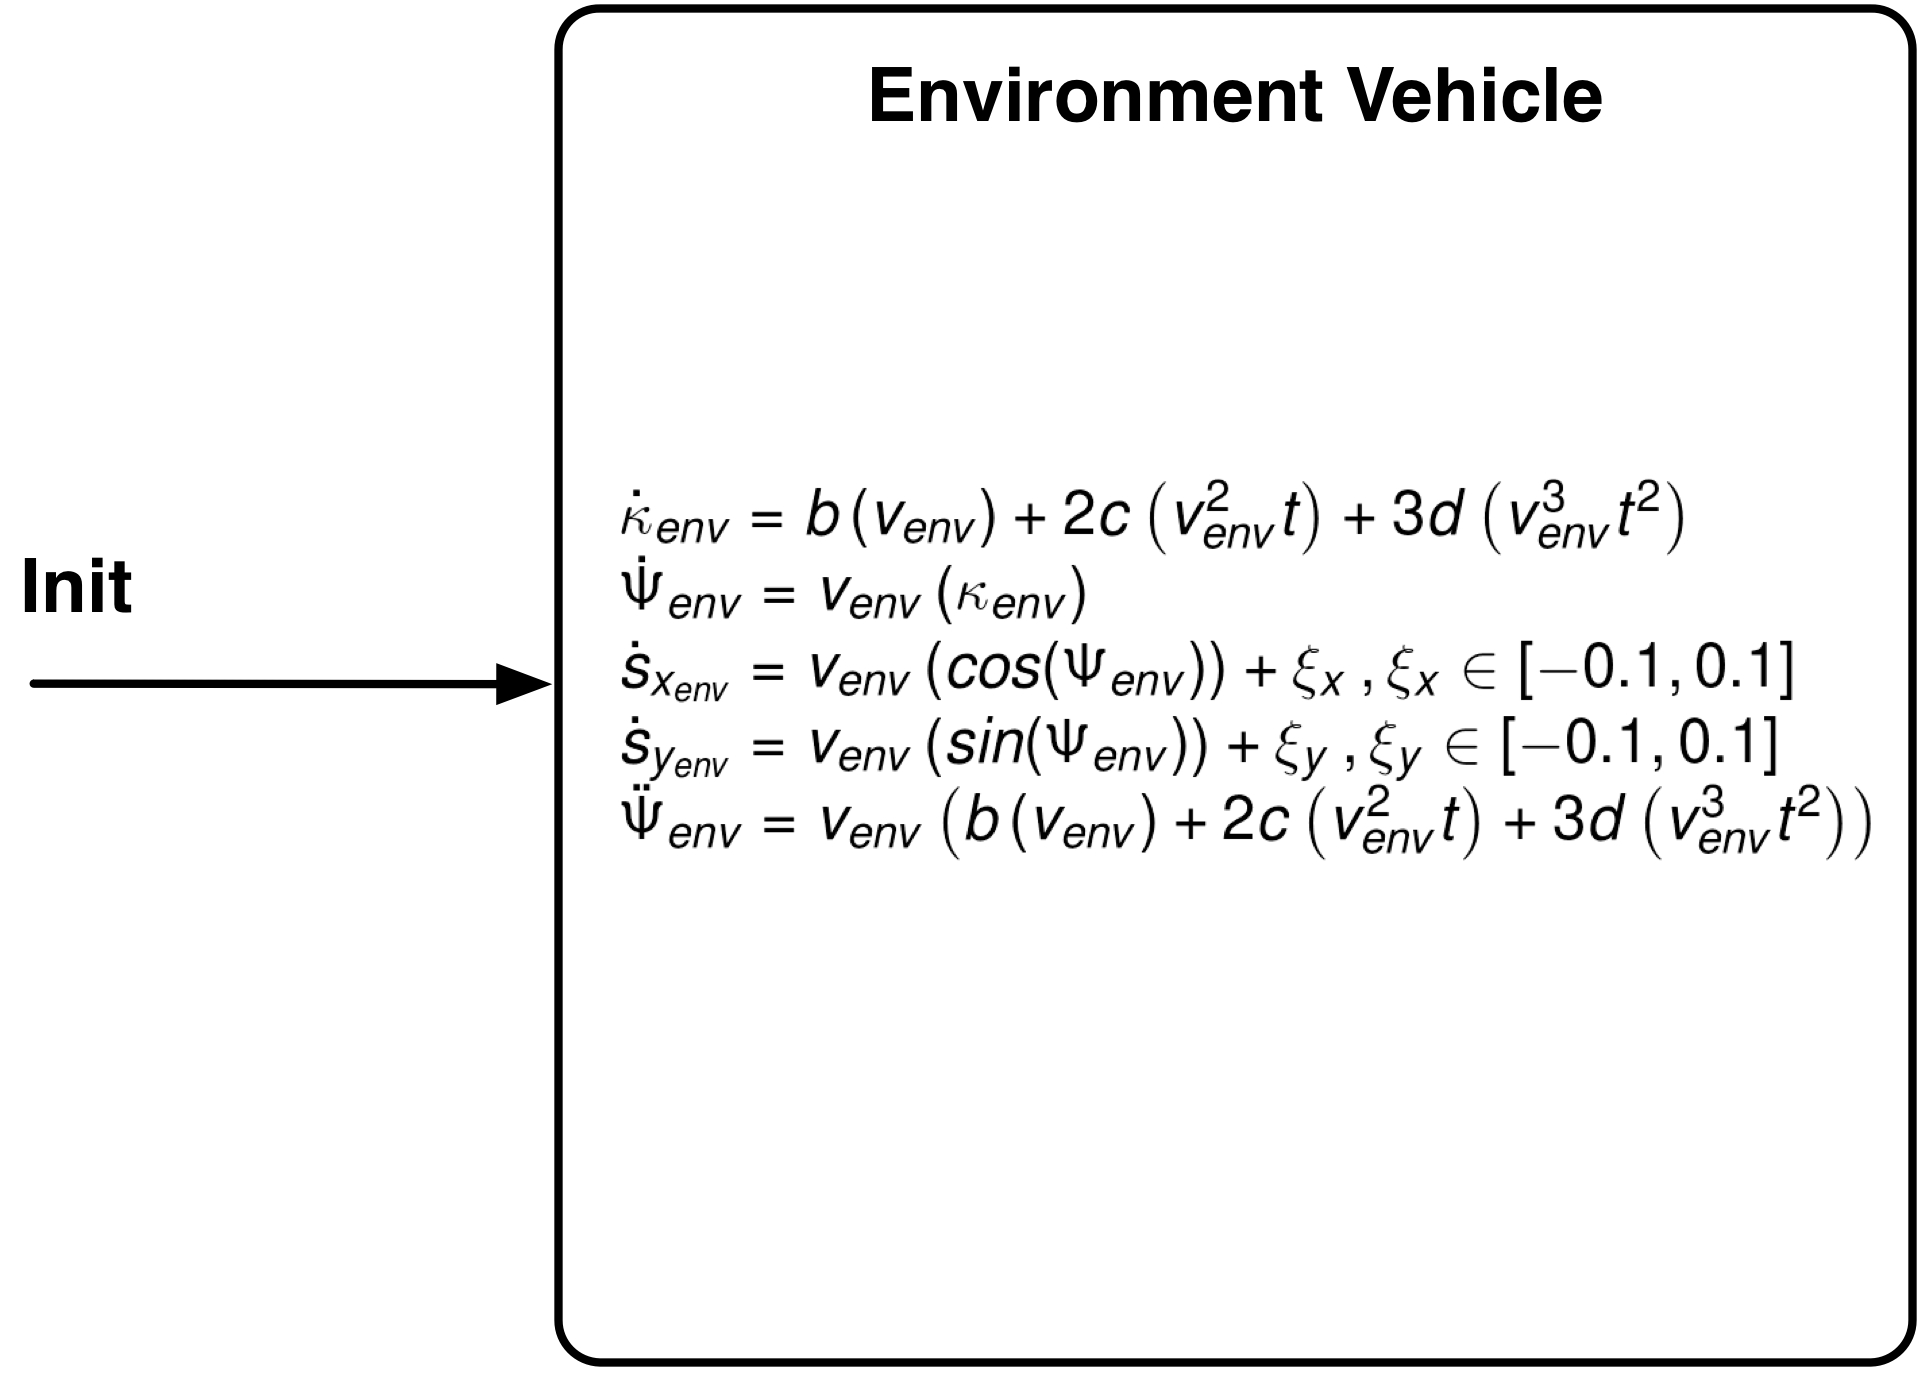
\includegraphics[scale=0.35]{figures/environment}
		\caption{Environment Vehicle Automaton}
	\end{figure}
The other vehicles operating within a scenario present both an interesting challenge and a primary motivation for formal verification. It is clear that it is impossible to know the intentions of the agents operating such vehicles; their execution represents a significant source of non-determinism. In fact, a more complex model of such agents which includes details such as steering angle or tire friction will not enable less conservative results, for it is the control input not the plant that remains the largest unknown. Thus, we conclude that:
{\it for verifying the autonomous agent, only the perceptible behavior of other agents is important, not their internal structure.}



Still it remains clear that {\it the behavior of other agents must be part of the scenario description.} As such we present a safety case which assumes that other agents will follow a certain minimal set of driving rules. For brevity we will reference the following specification as $\xi$ in the case studies.% as specified in \cite{Althoff2014} which is a subset of the Vienna Convention on Road Traffic \cite{Europe.TransportDivision2007}:

\begin{itemize}
	\item Acceleration ceases when some maximum velocity is reached.
	\begin{equation}
	\Box \left( v_{env} \geq v_{max} \to a = 0 \right)
	\end{equation}
	\item Other agents must drive in the proper direction according to their lane.
	\begin{equation}
	\Box \left( v_{env} \geq 0 \right)
	\end{equation}
	\item The accelerations of other agents are within those rates achievable by maximum engine power
	\begin{equation}
	\Box \left( a_{env} \leq a_{max}\right)
	\end{equation}
	\item Other agents maintain their lanes unless explicitly specified not to.
	\begin{equation}
	\Box \left( \neg LC \to \left( y_{min} \leq s_{y_{env}} \right) \wedge \left( y_{max} \geq s_{y_{env}} \right) \right)
	\end{equation}
	\item Lane changes by other agents are only permitted if the alternate lane is unoccupied or unless a degenerate scenario is being modeled.
	\begin{equation}
	\Box \left( LO \to \neg LC \right)
	\end{equation}
	

	
\end{itemize}

\section{Hybrid Model: Composition of Agents}
\subsection{Ego-Vehicle}
\subsection{Other Vehicles}
\subsection{Composition}
\subsection{General Complexity}


%------------------------------------------------------------------------------
\section{Benchmarks}
\subsection{A Simple Lane Change}
\begin{itemize}
	\item We first present this scenario in \cite{blah}
	\item Other authors \cite{blah} have considered with static obstacles
	\item Counterexamples are somewhat obvious
	\item Inductive invariance argument allows verification of infinite time properties
		\item Most examples involving forward safety are monotonic ie selecting a lower operating speed implies an decrease in stopping time and improves the forward safety of the vehicle. 
		\item In such problems there are no ``holes" in the interval. 
		\item Resulting proofs seem to indicate that testing would be sufficient to find counterexamples because unsafe results occur at extreme points in the state space only.
		\begin{itemize}
			\item Verification still provides a guarantee of safety that was not previously available. 
			\item Verification is still useful for formally verifying specifications and interaction between supplier systems and vehicle dynamics.
			\item Helps to search for viable combinations of specifications
		\end{itemize}
	\item We extend this scenario with differential inclusions. 
	\item Problem: we are forced into the tree representation because we cannot bring the trajectory generator in the dReach framework, requires external libraries and iteration. Could be remedied via creation of a lookup table or Neural Network. Alternative is to change the trajectory generation strategy such as Pure Pursuit.
\end{itemize}

\subsection{Algorithm}
How we establish safety of a decision controller.
\begin{algorithm}
	\caption{Check Trajectory Sequence}
	\label{algo:trajseq}
	\begin{algorithmic}
		\State \textbf{checkSequence} (searchDepth)
		\State  bool $safetyVar := TRUE$
		\State int $depth := 0$
		\While {$depth \leq searchDepth$}
		\State float* $trajectoryParam = getNextTrajectory(depth)$
		\State $safetyVar := checkTrajectory(trajectoryParam)$
		\State
		\EndWhile
		\State \Return {$safetyVar$}
	\end{algorithmic}
\end{algorithm}
Proofs and lemmas:
\textbf{For an appendix?}
\begin{theorem}
	Proof of compositional nature of safety of sequence of trajectories
\end{theorem}

\begin{theorem}
	Contract for parallel composition of verification instances
\end{theorem}

\begin{theorem}
	Inductive invariance for search termination at a specified depth. 
\end{theorem}


\subsection{Variations in Road Geometry}
%\textbf{Random Ideas, not to be taken seriously}
%\begin{itemize}
%	\item Can we think of a type theoretic description of configuration space rather than set theoretic?
%	\item For example think of configuration space as a type
%	\item Pose and Goal can then be considered points of the configuration space type 
%	\item There exists many paths between a single pose and goal pair, all of these paths are equivalent from a type theoretic perspective.
	%\item Narrow down an instance of these paths by describing a decision procedure necessary to generate the path ie pure pursuit or cubic splines, the type of these functions is a path between goal and pose. 
%\end{itemize}

\begin{itemize}
	\item In order to pursue more complex scenarios with more expressive agents we propose a variation in the trajectory generation strategy which admits a closed form
	\item Implement pure pursuit trajectory generation strategy...
\end{itemize}
\begin{itemize}

	\item Open question if we can guarantee infinite time properties in general case, or on road by road basis via inductive invariant. 
	\item A second question of interest is the scalability of results involving multiple agents and curved roads. 
	\item Pure Pursuit can be represented directly in the Hybrid Program and admits a closed form solution for curvature.
	\item Using a Hybrid program we now show how the number of paths through the state space grows exponentially with the addition of other agents and events as well as increases in search depth. 
\end{itemize}

We present a scenario as shown in Figure \ref{fig:scenario2}
\begin{figure}
	\centering
	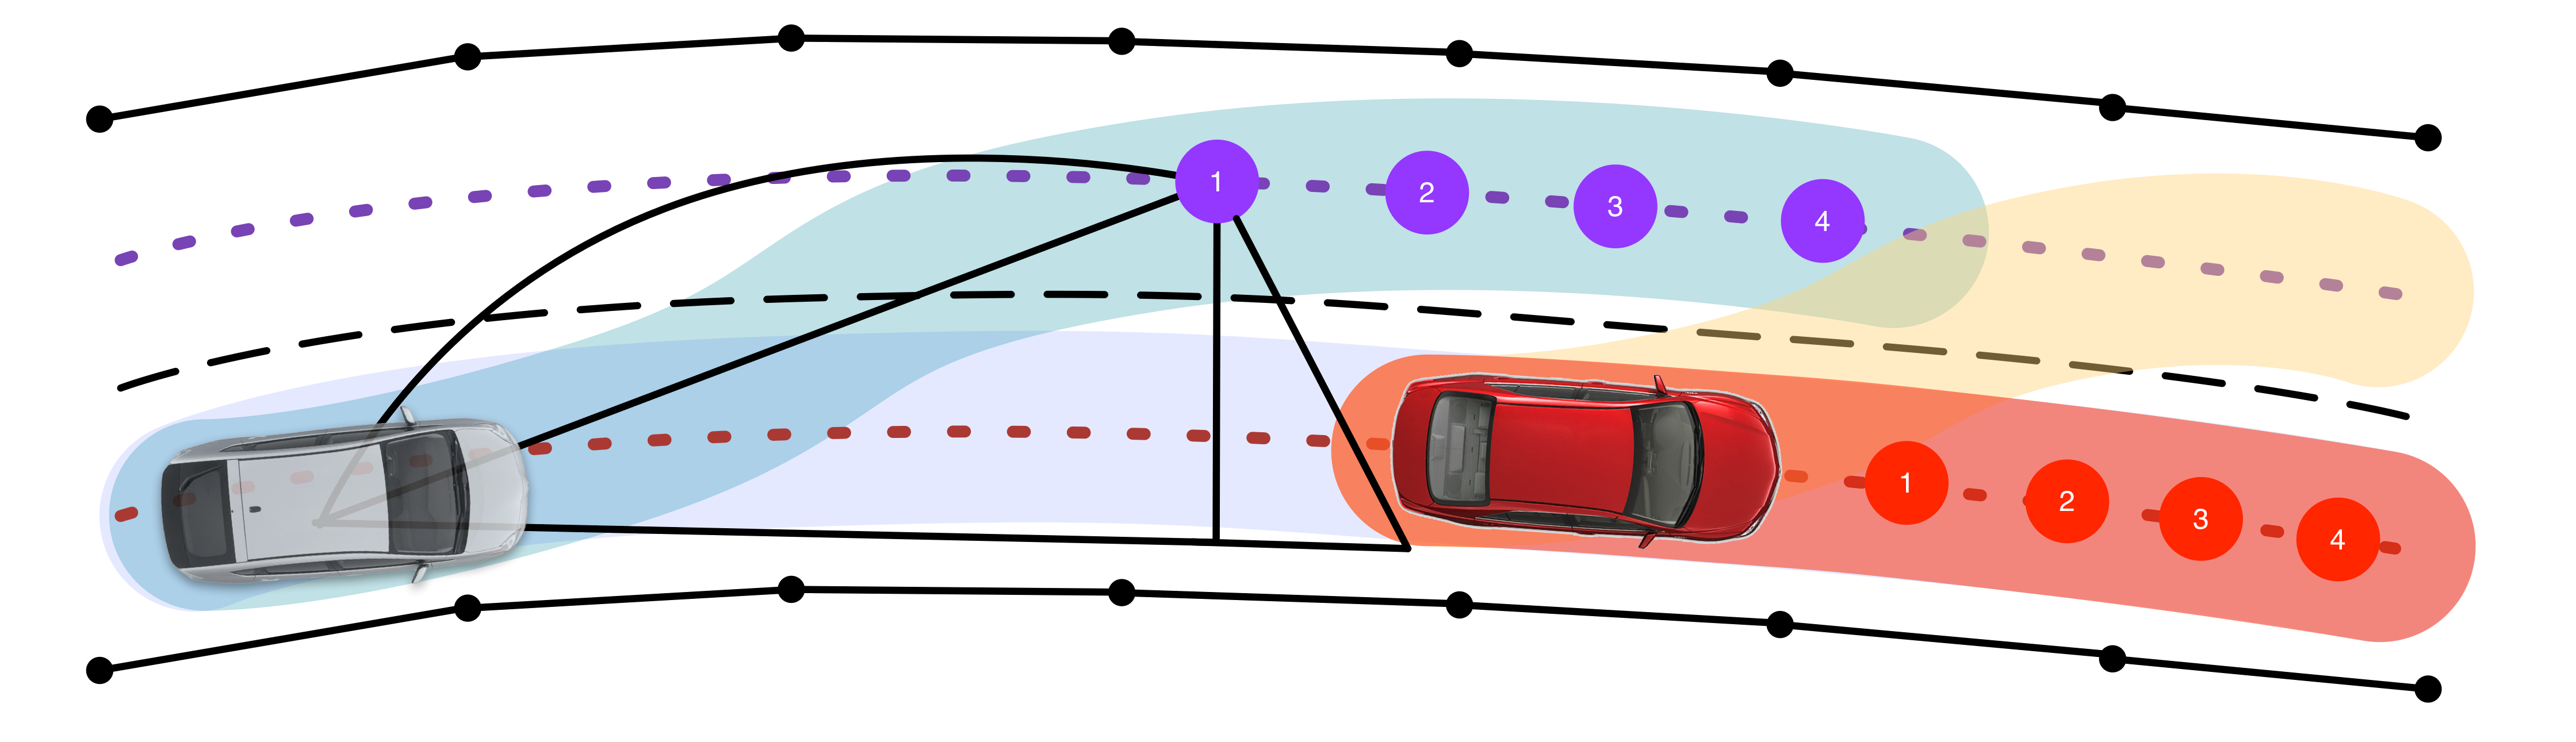
\includegraphics[scale=.4]{figures/scenario2}
	\caption{A graphical representation of the lane change scenario on a curved road}
\end{figure}
\begin{itemize}
	\item The previous example is the simplest possible instantiation of a lane change scenario
	\item Here we present an increasingly nuanced view of the the vehicle environment system
	\begin{itemize}
		\item Singleton inital sets and deterministic transitions
		\item Initial sets defined by intervals
		\item Non-determinism as applied to discrete decisions by the environment
		\item Automaton complexity in terms of states as number of agents grows
		\item Automaton complexity in terms of states as number of reference trajectories grows
		\item Search complexity in terms of path length as number of agents grows
		\item Search complexity in terms of path length as number of reference trajectories grows
		\item Non-deterministic scheduling of trajectory update
		\item Environment agents continuous dynamics are represented as differential inclusions (another form of non-determinism)
		\item Ego vehicle agents continuous dynamics are disturbed via errors represented as differntial inclusions
		\item Ego vehicle and environmental agents subjected to discrete events representing sensor or actuator failures.
	\end{itemize}
\end{itemize}
%------------------------------------------------------------------------------
\section{Conclusions}

	\begin{itemize}
		\item Types of Uncertainty:
		\begin{itemize}
			\item Scenario Configuration
			\item Initial Estimation Errors
			\item Noise in dynamics
			\item Sensor estimation errors
			\item Sensing thresholds
		\end{itemize}
	\end{itemize}
	\begin{itemize}
		\item Scenario 1: Lane change on straight road with two agents
		
		\item Scenario 2: Curved road with hybrid program representation
		\begin{itemize}
			\item No longer have clear invariant cut
		\end{itemize}
		\item Scenario 3: Four way intersection governed by a traffic light
		\begin{itemize}
			\item Map provides knowledge of obstruction and automatically adjusts behavior
		\end{itemize}
		\begin{itemize}
			\item Variant: Traffic light
			\item Variant: Pedestrian
		\end{itemize}
	\end{itemize}


\label{sect:bib}
\bibliographystyle{plain}
%\bibliographystyle{alpha}
%\bibliographystyle{unsrt}
%\bibliographystyle{abbrv}
\bibliography{easychair}

\begin{comment}
%------------------------------------------------------------------------------
\appendix
\section{Formatting Information}
\label{sect:easychair-requirements}
\begin{enumerate}
	\item
	The default paper size is US letter. It can be explicitly set to A4 
	(\texttt{a4paper}) or letter (\texttt{letterpaper}) paper in the
	document class entry, e.g.:\\\verb+\documentclass[a4paper]{easychair}+
	
	\item
	The print area for both letter and A4 paper sizes is 145x224 mm. This size
	has been selected to allow for inexpensive printing using our current
	print-on-demand publisher.
	
	\item
	The base font is Computer Modern. The base font size is 10pt. If you
	use any other font size, there is no guarantee that the produced
	document will look nice or fit into our standard page size.
	
	\item
	The references list is condensed. The default bibliography styles, such as
	\texttt{plain}, \texttt{abbrv}, and \texttt{alpha}, are suggested.
	
	\item
	PNG, JPG, and PDF images are supported, i.e., those that are supported
	by the standard \texttt{graphicx} package \cite{graphicx-package}, and
	render nicely in online versions of PDF documents.  This document
	shows some examples of JPG and PDF images, for example in
	Figure~\ref{fig:easychair-logo}. If the papers are designed for
	publishing in print, the images should be at least 300dpi in
	resolution. 
	
\end{enumerate}

\subsection{Tables}

Many page overflows happen because of large tables. In many case these
overflows can be easily removed by slightly reducing padding added by
\LaTeX\ to every column. It is controlled by the \LaTeX\ command
\verb|\tabcolsep| whose value by default is 6pt. Even small changes in
the value of this command may give drastic reductions in the width of
tables. This is illustrated in Figure~\ref{fig:tabcolsep} on
page~\pageref{fig:tabcolsep}. Note though that there is no free lunch:
smaller values for this command may result in lower redability.

%------------------------------------------------------------
\begin{figure}[tb]\small
	\begin{center}
		\begin{tabular}{lrrrrrrrr}
			\hline
			ATP System            & LTB & Avg  &Prfs & SOTA & \multicolumn{1}{c}{$\mu$} & CYC & MZR & SMO \\
			\hline
			Vampire-LTB 11.0      &  69 & 24.5 &  69 & 0.37 & 28.1 &  23 &  22 &  24 \\
			iProver-SInE 0.7      &  67 & 76.5 &   0 & 0.36 &  8.8 &  28 &  14 &  25 \\
			\hline
		\end{tabular}
	\end{center}
	
	\begin{center}\renewcommand{\tabcolsep}{5pt}
		\begin{tabular}{lrrrrrrrr}
			\hline
			ATP System            & LTB & Avg  &Prfs & SOTA & \multicolumn{1}{c}{$\mu$} & CYC & MZR & SMO \\
			\hline
			Vampire-LTB 11.0      &  69 & 24.5 &  69 & 0.37 & 28.1 &  23 &  22 &  24 \\
			iProver-SInE 0.7      &  67 & 76.5 &   0 & 0.36 &  8.8 &  28 &  14 &  25 \\
			\hline
		\end{tabular}
	\end{center}
	
	\begin{center}\renewcommand{\tabcolsep}{3pt}
		\begin{tabular}{lrrrrrrrr}
			\hline
			ATP System            & LTB & Avg  &Prfs & SOTA & \multicolumn{1}{c}{$\mu$} & CYC & MZR & SMO \\
			\hline
			Vampire-LTB 11.0      &  69 & 24.5 &  69 & 0.37 & 28.1 &  23 &  22 &  24 \\
			iProver-SInE 0.7      &  67 & 76.5 &   0 & 0.36 &  8.8 &  28 &  14 &  25 \\
			\hline
		\end{tabular}
	\end{center}
	
	\begin{center}\renewcommand{\tabcolsep}{1pt}
		\begin{tabular}{lrrrrrrrr}
			\hline
			ATP System            & LTB & Avg  &Prfs & SOTA & \multicolumn{1}{c}{$\mu$} & CYC & MZR & SMO \\
			\hline
			Vampire-LTB 11.0      &  69 & 24.5 &  69 & 0.37 & 28.1 &  23 &  22 &  24 \\
			iProver-SInE 0.7      &  67 & 76.5 &   0 & 0.36 &  8.8 &  28 &  14 &  25 \\
			\hline
		\end{tabular}
	\end{center}
	\normalsize
	
	\caption{Original table and tables with \texttt{tabcolsep} set to 5pt,
		3pt, and 1pt
		\label{fig:tabcolsep}}
	
\end{figure}
%------------------------------------------------------------

\subsection{Images}

Images included using \verb|\includegraphics| are easy to resize since
one can specify the size of the result explicitly. For example,
Figure~\ref{fig:easythrone} shows three copies of the same image
having different sizes obtained using the following commands:

\begin{verbatim}
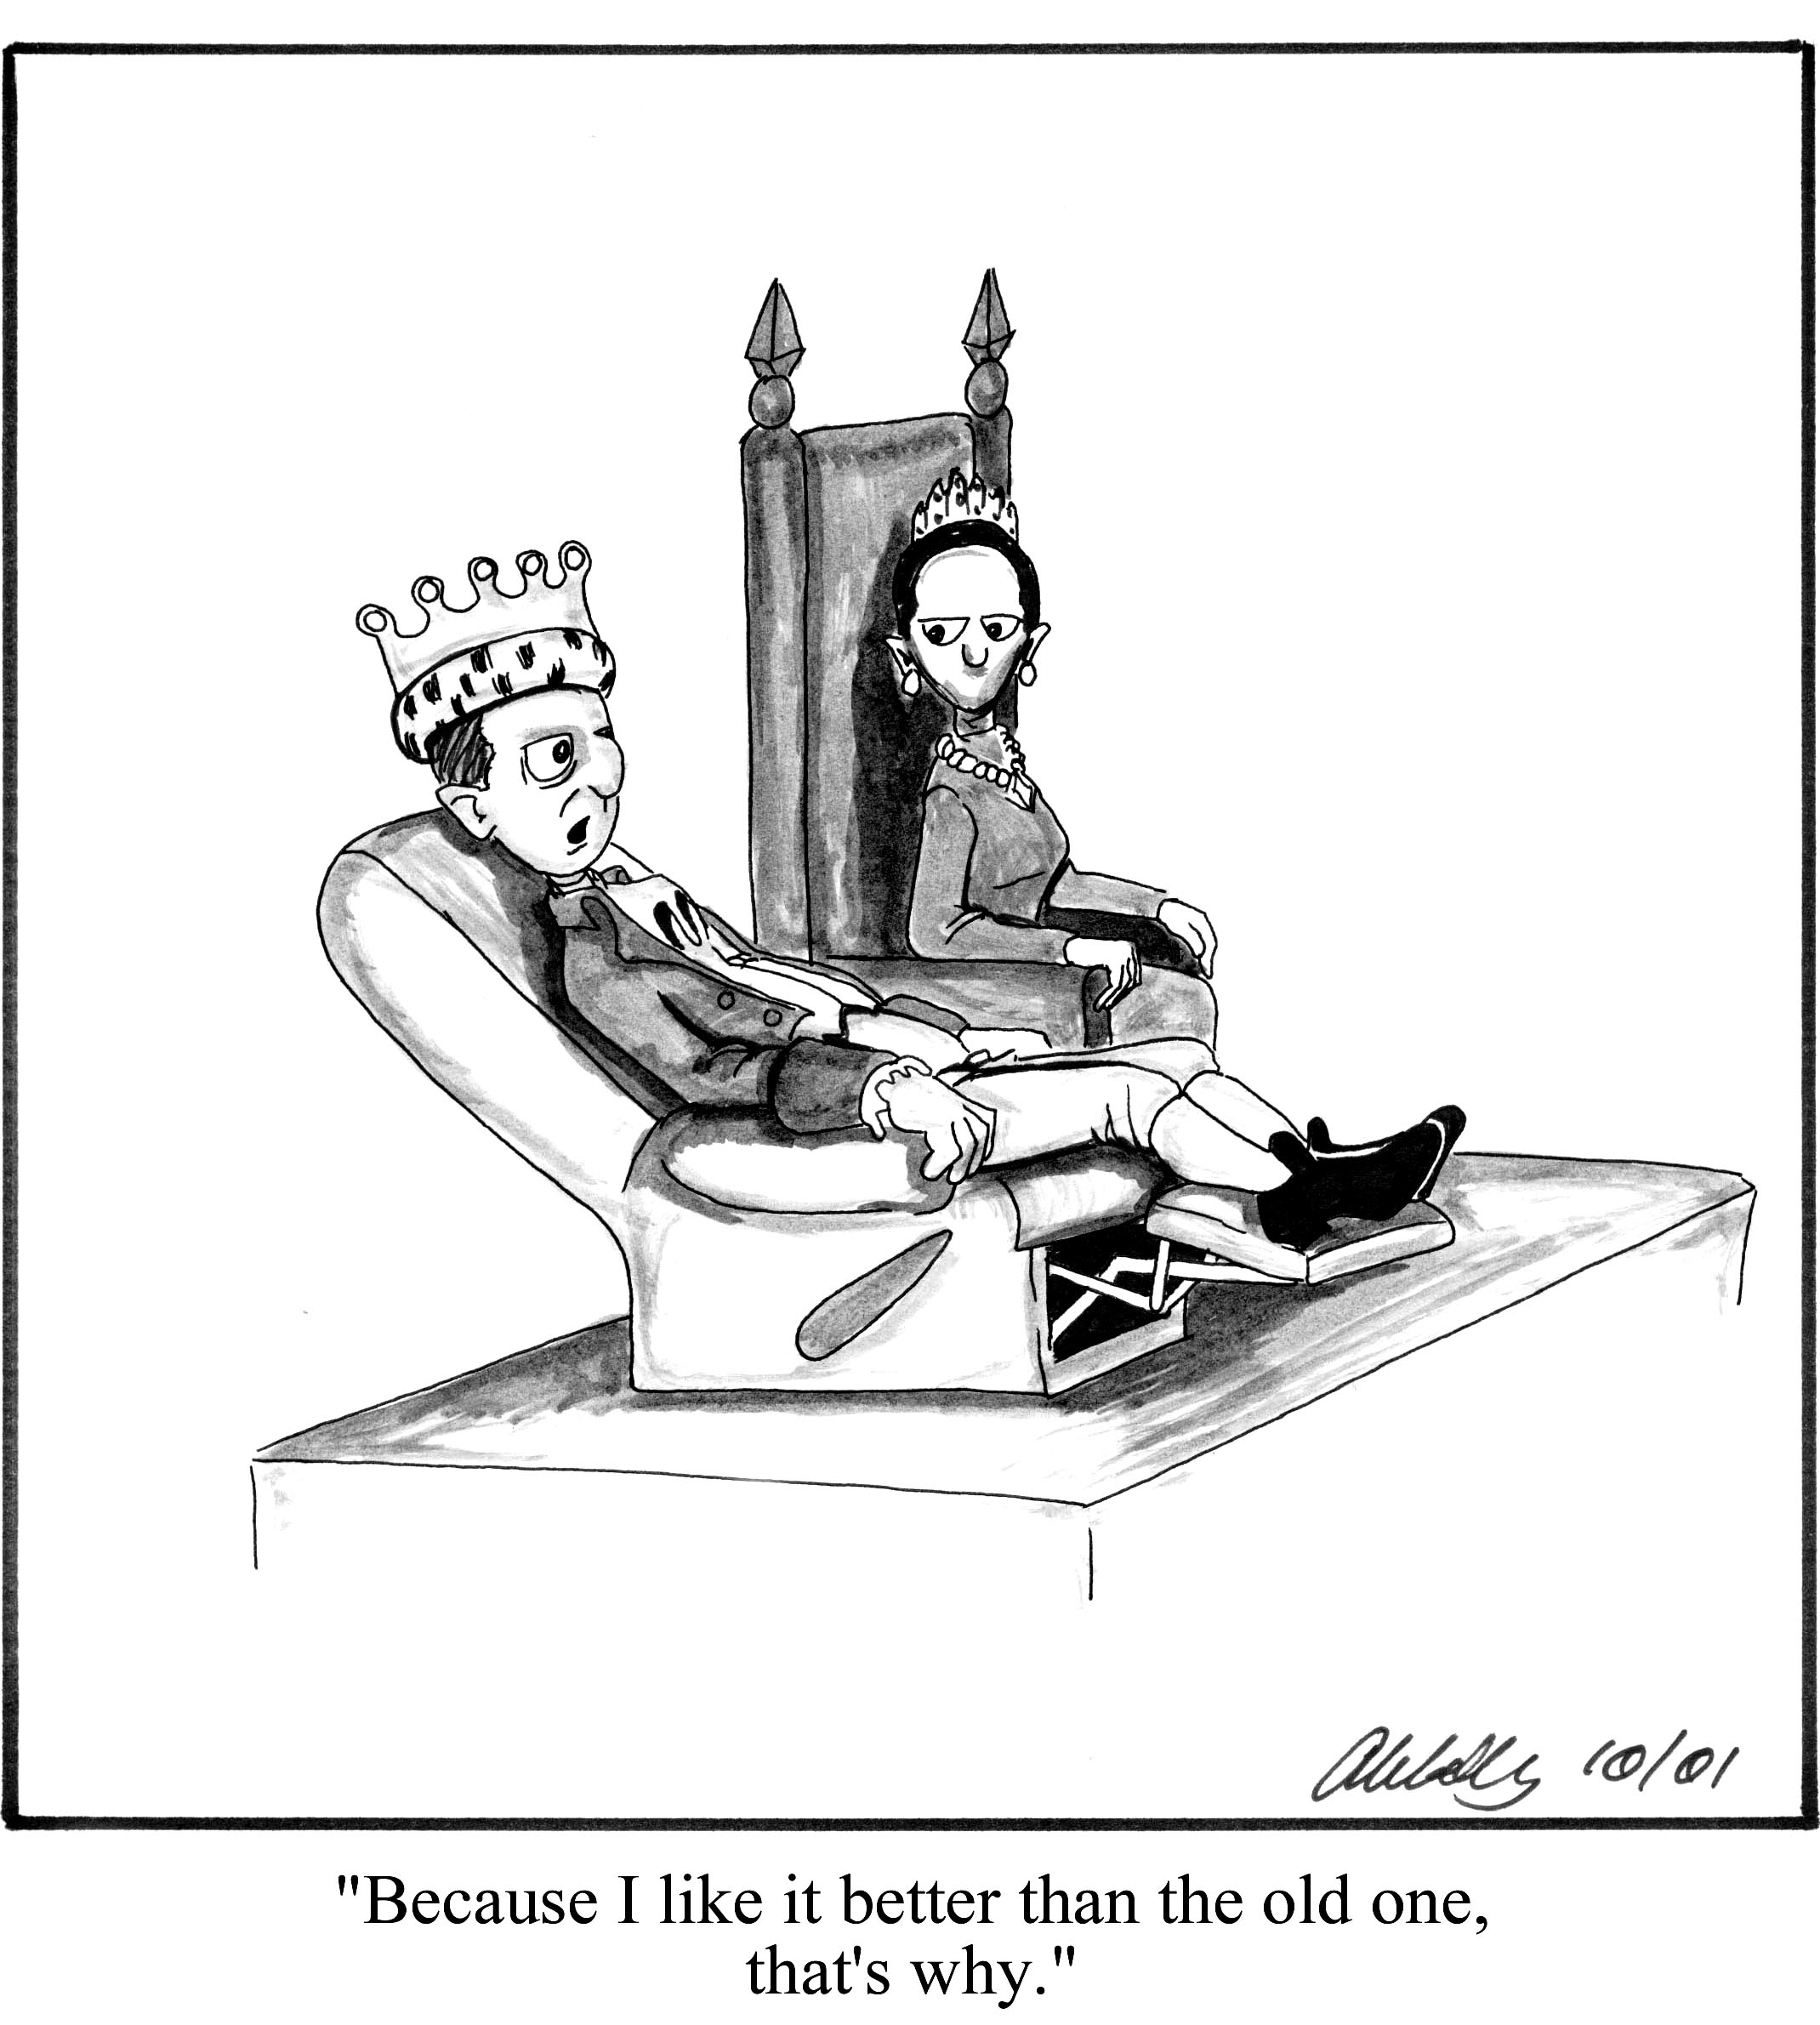
\includegraphics[width=0.5\textwidth]{throneEC.jpg}
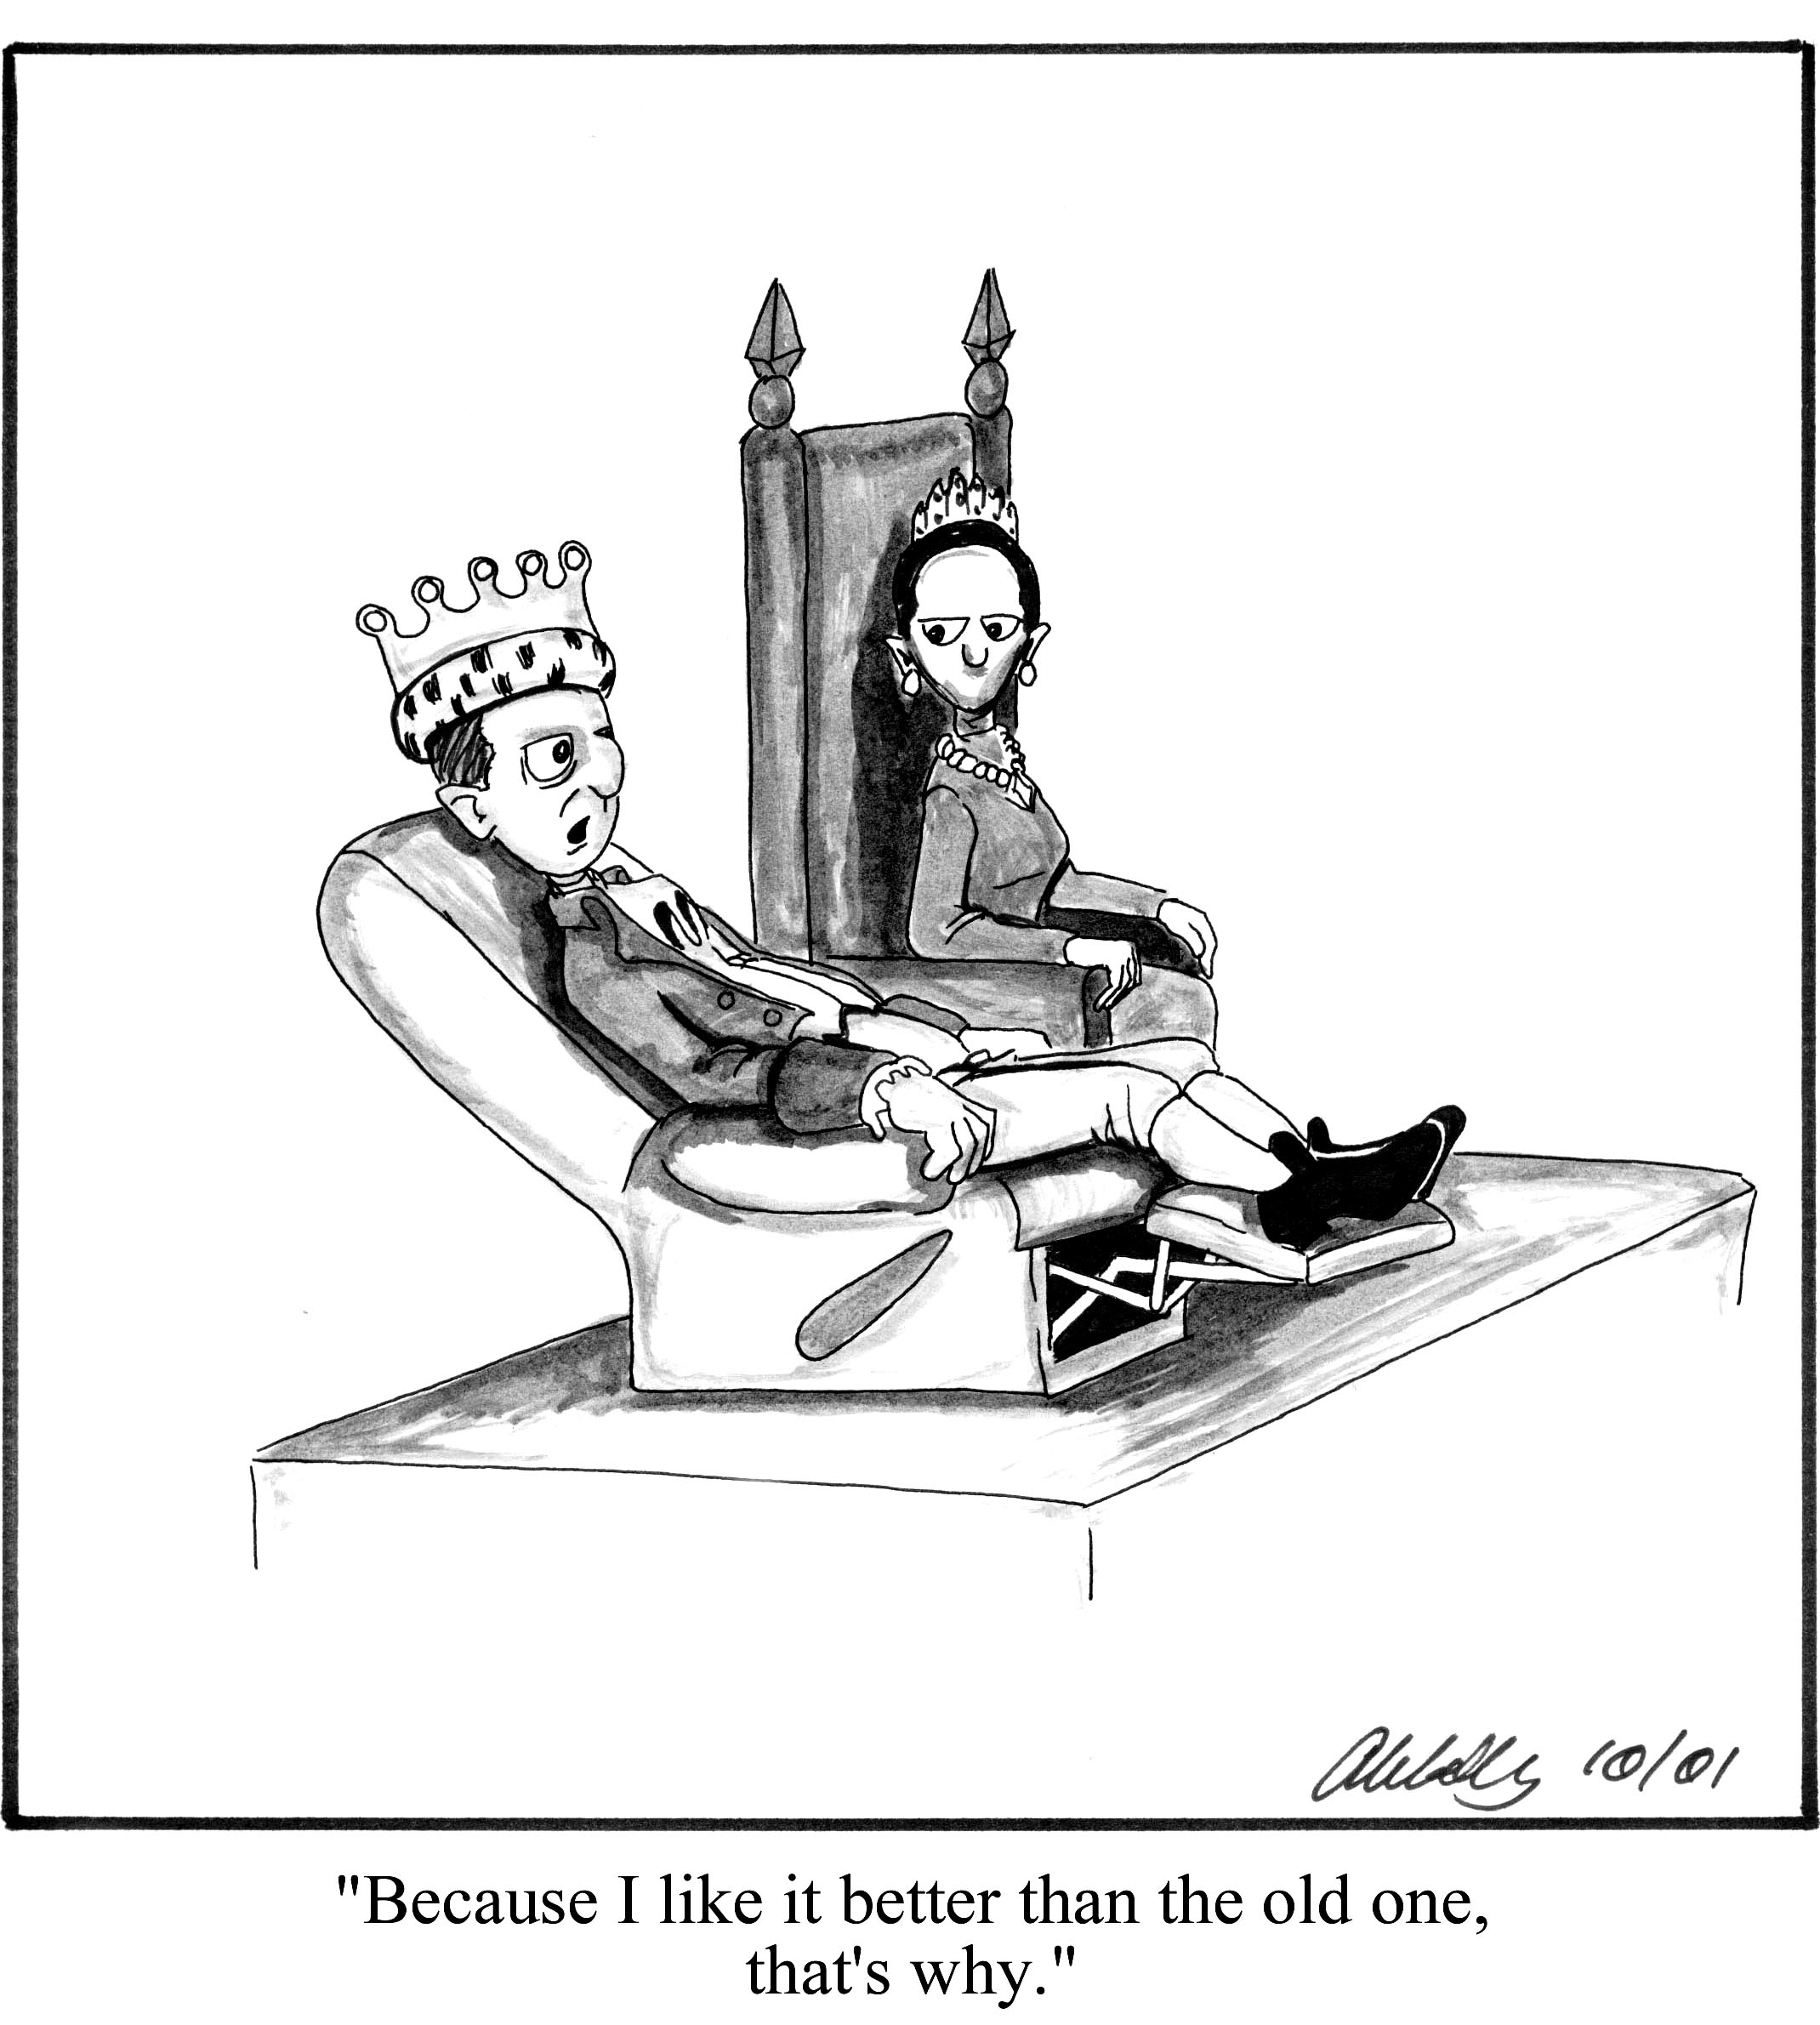
\includegraphics[width=0.3\textwidth]{throneEC.jpg}
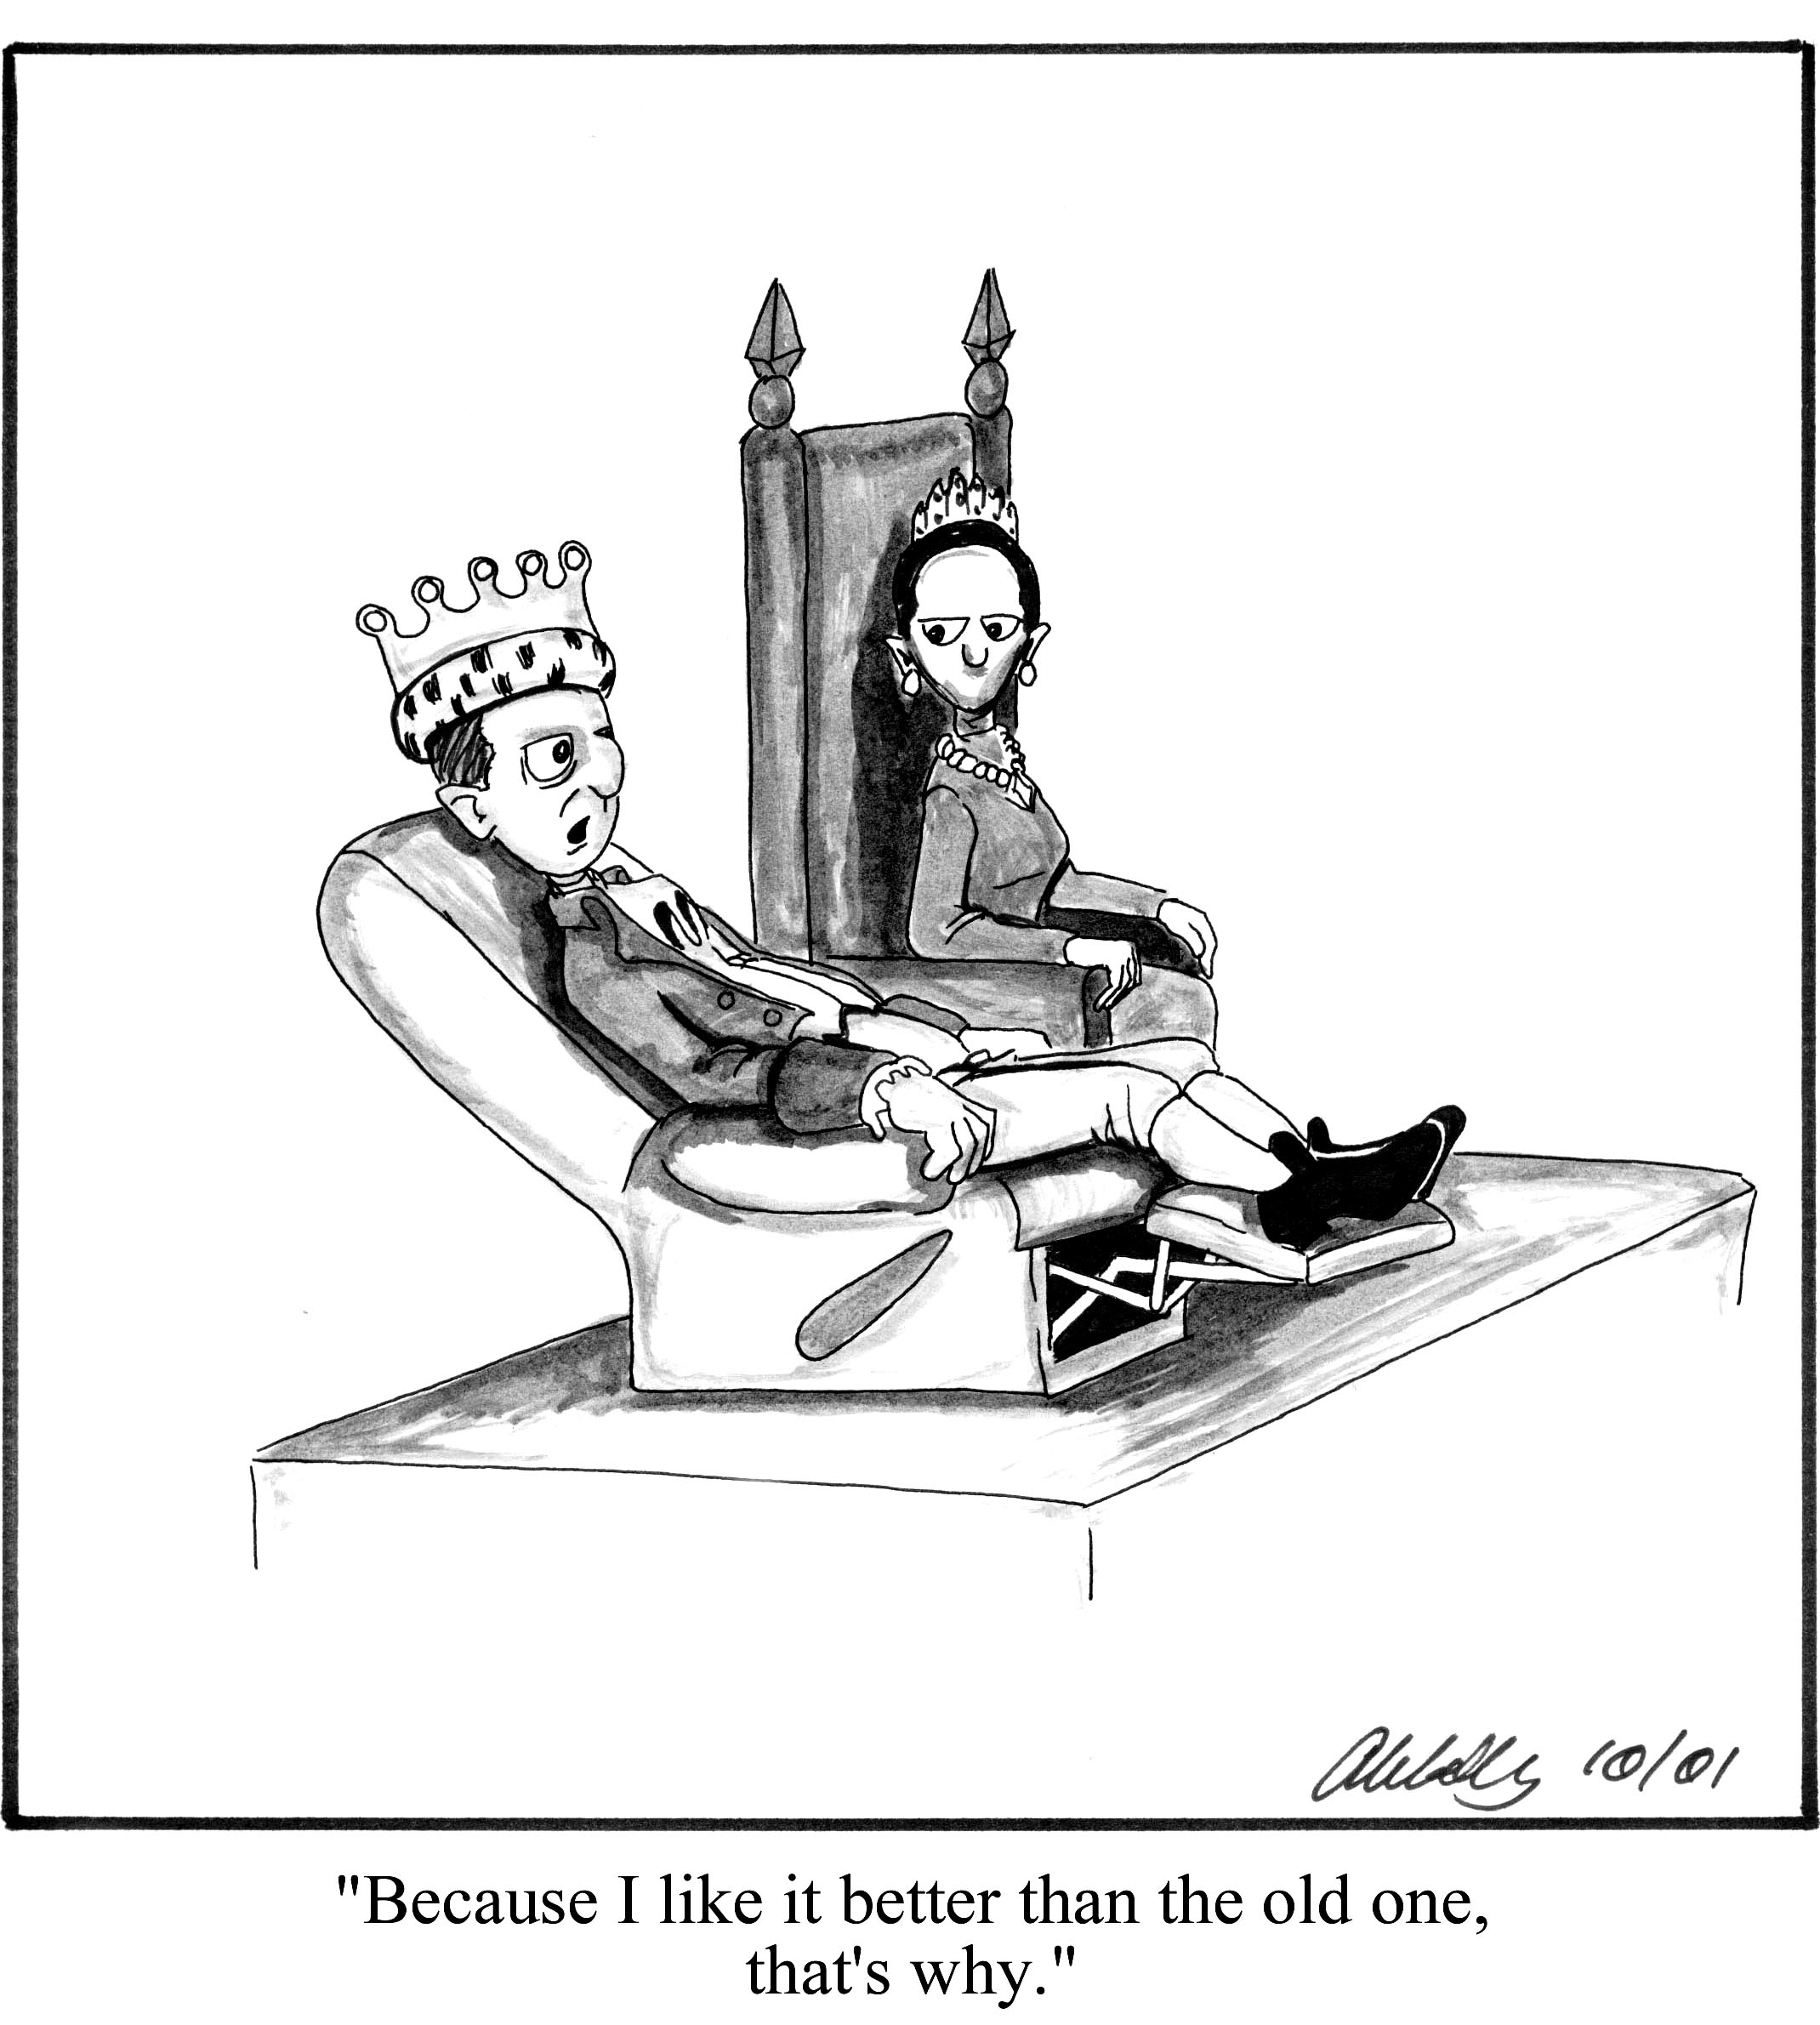
\includegraphics[width=0.15\textwidth]{throneEC.jpg}
\end{verbatim}

\subsection{A Universal Recipe}

\LaTeX\ has a very powerful weapon for reducing the size of almost
anythings. More precisely, it can reduce anything producing what
\LaTeX\ considers a box. This weapon is called
\verb|\scalebox|. Consider an example (check the source of this file
to see how it was produced).

\begin{center}
	\begin{tabular}{|c|c|}
		\hline \Huge
		\begin{tabular}[b]{cr}
			year & users \\ \hline
			2007 &    47,753 \\
			2008 &    114,494 \\
			2009 &    207,506 \\
			2010 &   371,054 \\
		\end{tabular}
		&
		
\includegraphics[width=0.28\textwidth]{chairEC}\\
		\hline
		\multicolumn{2}{|c|}{The number of users of EasyChair and one of its
			logos,}\\
		\multicolumn{2}{|c|}{scaled to the number of users in 2010} \\
		\hline
	\end{tabular}
\end{center}
This is what happens when we put (almost) the same \LaTeX\ code in 
\verb|\scalebox{0.55923}{...}| to scale it down to the number of users
in 2009:

\begin{center}
	\scalebox{0.55923}{%
		\begin{tabular}{|c|c|}
			\hline \Huge
			\begin{tabular}[b]{cr}
				year & users \\ \hline
				2007 &    47,753 \\
				2008 &    114,494 \\
				2009 &    207,506 \\
				2010 &   371,054 \\
			\end{tabular}
			&
			
\includegraphics[width=0.28\textwidth]{chairEC}\\
			\hline
			\multicolumn{2}{|c|}{The number of users of EasyChair and one of its
				logos,}\\
			\multicolumn{2}{|c|}{scaled to the number of users in 2009} \\
			\hline
		\end{tabular}}
	\end{center}
	We can scale it down even further to the 2008 figure using
	\verb|\scalebox{0.30856}{...}|:
	
	\begin{center}
		\scalebox{0.30856}{%
			\begin{tabular}{|c|c|}
				\hline \Huge
				\begin{tabular}[b]{cr}
					year & users \\ \hline
					2007 &    47,753 \\
					2008 &    114,494 \\
					2009 &    207,506 \\
					2010 &   371,054 \\
				\end{tabular}
				&
				
\includegraphics[width=0.28\textwidth]{chairEC}\\
				\hline
				\multicolumn{2}{|c|}{The number of users of EasyChair and one of its
					logos,}\\
				\multicolumn{2}{|c|}{scaled to the number of users in 2008} \\
				\hline
			\end{tabular}}
		\end{center}
		or further down to 2007:
		
		\begin{center}
			\scalebox{0.12870}{%
				\begin{tabular}{|c|c|}
					\hline \Huge
					\begin{tabular}[b]{cr}
						year & users \\ \hline
						2007 &    47,753 \\
						2008 &    114,494 \\
						2009 &    207,506 \\
						2010 &   371,054 \\
					\end{tabular}
					&
					
\includegraphics[width=0.28\textwidth]{chairEC}\\
					\hline
					\multicolumn{2}{|c|}{The number of users of EasyChair and one of its
						logos,}\\
					\multicolumn{2}{|c|}{scaled to the number of users in 2008} \\
					\hline
				\end{tabular}}
			\end{center}
			
			This size reduction technique is very efficient: using the right scale
			you may post your whole article on Twitter in a single tweet. However,
			it may also may parts of your text virtually unreadable with an
			unfortunate side effect of annoying reviewers. 
\end{comment}

%------------------------------------------------------------------------------
% Index
%\printindex

%------------------------------------------------------------------------------
\end{document}

% EOF
